		\documentclass{minimal}
		\usepackage{dozenal}
		\usepackage{lettrine}
		\usepackage{xfrac}
		\usepackage[absolute,overlay]{textpos}
		\usepackage[T1]{fontenc}
		\usepackage{lmodern} \normalfont
		\DeclareFontShape{T1}{lmr}{bx}{sc} { <-> ssub * cmr/bx/sc }{}
		\usepackage{array}
		\usepackage{lscape}
		\usepackage{calc}
		\usepackage{tcolorbox}
		\usepackage{booktabs}
		\usepackage{multicol}
		\usepackage{pdfpages}
		\usepackage{ifthen}
		\usepackage{graphicx}
		\usepackage{textcomp}
		\usepackage{url}
		\newlength{\shortline}
		\newlength{\thirdskip}
		\newlength{\weeklydayboxwid}
		\setlength\arrayrulewidth{.4pt}
		\setlength\extrarowheight{4pt}
		\usepackage[paperwidth=8.5in,paperheight=11in,width=7.5in,height=10.5in,bottom=0.25in]{geometry}
		\usepackage{lscape}
		\usepackage{graphicx}
		\usepackage{eso-pic}
		\usepackage{calc}
		\usepackage{transparent}
		\def\Biggie{\fontsize{17pt}{19pt}\selectfont}
		\def\Big{\fontsize{14pt}{17pt}\selectfont}
		\def\yearlytitsty{\fontsize{18pt}{18pt}\selectfont\bfseries}
		\def\tabheadsty{\bfseries\scshape}
		\def\timesty{\fontsize{10pt}{12pt}\selectfont}
		\def\copypagesty{\fontsize{12pt}{12pt}\selectfont}
		\def\monthsty#1{\fontsize{36pt}{40pt}\textsc{#1}}
		\def\weektitlsty{\fontsize{24pt}{24pt}\selectfont\scshape}
		\def\thumbtitsty{\fontsize{11pt}{11pt}\selectfont\bfseries\scshape}
		\def\weekletsty{\fontsize{8pt}{8pt}\selectfont}
		\def\daysty{\centering\Biggie\scshape}
		\def\weekdaysty{\centering\scshape}
		\def\eventsty{\fontsize{9pt}{9pt}\itshape}
		\def\numsty{\fontsize{14pt}{16pt}\selectfont}
		\def\smallnum{\fontsize{10pt}{10pt}\selectfont\bfseries}
		\def\extsmall{\fontsize{7pt}{7pt}\selectfont\bfseries}
		\def\feaststy#1{\vbox{\centering\scshape\fontsize{11pt}{12pt}\selectfont#1}}
		\def\halffeast#1{\vbox{\centering\scshape\fontsize{10pt}{11pt}\selectfont#1}}
		\def\classsty#1{\vspace{-0.5em}\vbox{\centering\scshape\fontsize{9pt}{10pt}\selectfont#1}}
		\def\halfclass#1{\vspace{\fill}\scshape\fontsize{8pt}{10pt}\selectfont#1}
		\def\commsty#1{\vskip-.5em\vbox{\centering\upshape\fontsize{8pt}{9pt}\selectfont#1}}
		\def\halfcomm#1{\upshape\fontsize{9pt}{10pt}\selectfont#1}
		\def\colorsty#1{\vbox to\fill{\vfill\hbox to\linewidth{\hfill\itshape\fontsize{8pt}{10pt}\selectfont#1\hfill}}}
		\def\halfcolor#1{\itshape\fontsize{8pt}{10pt}\selectfont#1}
		\def\ls{\hskip0.2em}
		\def\shorts{\hskip0.1em}
		\begin{document}
		\newlength\daywidth
		\setlength{\daywidth}{10in/7 - 3.19986pt/7}
		\newlength{\smallday}
		\setlength{\smallday}{1.3em}
		\newlength\boxwidth
		\setlength{\boxwidth}{10in/7 - 2pt}
		\newlength\dayheight
		\setlength{\dayheight}{6.7in/7}
		\newlength{\smallheight}
		\setlength{\smallheight}{0em}
		\def\specstyl#1{\centering\fontsize{10pt}{12pt}\selectfont\itshape #1}
		\setlength\parindent{0em}
		\setlength\shortline{\linewidth-6ex-9pt}
		\setlength\thirdskip{\shortline/3}
		\setlength\weeklydayboxwid{\linewidth+1pt}
		\setlength{\TPVertModule}{\baselineskip}
		\setlength{\TPHorizModule}{\thirdskip}

\begin{landscape}%
\vspace*{\stretch{1}}%
\fontsize{84pt}{84pt}\selectfont%
\hbox to\linewidth{C A L E N D A R}%
\hbox to\linewidth{\hskip2em F O R\hskip1em 	1\ 1\ \e\ 9\ \hskip2em}%
\vspace*{\stretch{1}}%
\vbox to0pt{%
\fontsize{18pt}{18pt}\selectfont%
\hbox to\linewidth{%
	\hfil\scshape The Dozenal Society of America\hfil}%
\hbox to\linewidth{%
	\hfil\url{http://www.dozenal.org}\hfil}%
}%
\newlength{\logowidth}%
\settowidth{\logowidth}{
\includegraphics[scale=0.7]{new_logo.png}}%%
\makeatletter%
%
\AddToShipoutPicture*{%%
\setlength{\@tempdimb}{0.24\paperwidth}%%
\setlength{\@tempdimc}{0.32\paperheight}%%
\setlength{\unitlength}{1pt}%%
\put(\strip@pt\@tempdimb,\strip@pt\@tempdimc){%
\hbox{\transparent{0.2}
\includegraphics[angle=90,scale=3]{new_logo.png}}%
}%
}%
\makeatother%
\end{landscape}%
\newsavebox{\monthnegtwo}
\savebox{\monthnegtwo}[\smallday]{%
\vbox to1em{\hbox{%
\setlength\extrarowheight{0pt}
\renewcommand*{\arraystretch}{0.2}
\begin{tabular}{p{\smallday}|p{\smallday}|%
p{\smallday}|p{\smallday}|p{\smallday}|p{\smallday}|%
p{\smallday}}
\multicolumn{4}{c|}{} &
\vbox to\smallheight {\hbox to \linewidth{\hfil\smallnum 1\hfil}
\rule{0pt}{\smallheight}}&\vbox to\smallheight {\hbox to \linewidth{\hfil\smallnum 2\hfil}
\rule{0pt}{\smallheight}}&\vbox to\smallheight {\hbox to \linewidth{\hfil\smallnum 3\hfil}
\rule{0pt}{\smallheight}}\\\hline
\vbox to\smallheight {\hbox to \linewidth{\hfil\smallnum 4\hfil}
\rule{0pt}{\smallheight}}&\vbox to\smallheight {\hbox to \linewidth{\hfil\smallnum 5\hfil}
\rule{0pt}{\smallheight}}&\vbox to\smallheight {\hbox to \linewidth{\hfil\smallnum 6\hfil}
\rule{0pt}{\smallheight}}&\vbox to\smallheight {\hbox to \linewidth{\hfil\smallnum 7\hfil}
\rule{0pt}{\smallheight}}&\vbox to\smallheight {\hbox to \linewidth{\hfil\smallnum 8\hfil}
\rule{0pt}{\smallheight}}&\vbox to\smallheight {\hbox to \linewidth{\hfil\smallnum 9\hfil}
\rule{0pt}{\smallheight}}&\vbox to\smallheight {\hbox to \linewidth{\hfil\smallnum \x\hfil}
\rule{0pt}{\smallheight}}\\\hline
\vbox to\smallheight {\hbox to \linewidth{\hfil\smallnum \e\hfil}
\rule{0pt}{\smallheight}}&\vbox to\smallheight {\hbox to \linewidth{\hfil\smallnum 10\hfil}
\rule{0pt}{\smallheight}}&\vbox to\smallheight {\hbox to \linewidth{\hfil\smallnum 11\hfil}
\rule{0pt}{\smallheight}}&\vbox to\smallheight {\hbox to \linewidth{\hfil\smallnum 12\hfil}
\rule{0pt}{\smallheight}}&\vbox to\smallheight {\hbox to \linewidth{\hfil\smallnum 13\hfil}
\rule{0pt}{\smallheight}}&\vbox to\smallheight {\hbox to \linewidth{\hfil\smallnum 14\hfil}
\rule{0pt}{\smallheight}}&\vbox to\smallheight {\hbox to \linewidth{\hfil\smallnum 15\hfil}
\rule{0pt}{\smallheight}}\\\hline
\vbox to\smallheight {\hbox to \linewidth{\hfil\smallnum 16\hfil}
\rule{0pt}{\smallheight}}&\vbox to\smallheight {\hbox to \linewidth{\hfil\smallnum 17\hfil}
\rule{0pt}{\smallheight}}&\vbox to\smallheight {\hbox to \linewidth{\hfil\smallnum 18\hfil}
\rule{0pt}{\smallheight}}&\vbox to\smallheight {\hbox to \linewidth{\hfil\smallnum 19\hfil}
\rule{0pt}{\smallheight}}&\vbox to\smallheight {\hbox to \linewidth{\hfil\smallnum 1\x\hfil}
\rule{0pt}{\smallheight}}&\vbox to\smallheight {\hbox to \linewidth{\hfil\smallnum 1\e\hfil}
\rule{0pt}{\smallheight}}&\vbox to\smallheight {\hbox to \linewidth{\hfil\smallnum 20\hfil}
\rule{0pt}{\smallheight}}\\\hline
\vbox to\smallheight {\hbox to \linewidth{\hfil\smallnum 21\hfil}
\rule{0pt}{\smallheight}}&\vbox to\smallheight {\hbox to \linewidth{\hfil\smallnum 22\hfil}
\rule{0pt}{\smallheight}}&\vbox to\smallheight {\hbox to \linewidth{\hfil\smallnum 23\hfil}
\rule{0pt}{\smallheight}}&\vbox to\smallheight {\hbox to \linewidth{\hfil\smallnum 24\hfil}
\rule{0pt}{\smallheight}}&\vbox to\smallheight {\hbox to \linewidth{\hfil\smallnum 25\hfil}
\rule{0pt}{\smallheight}}&\vbox to\smallheight {\hbox to \linewidth{\hfil\smallnum 26\hfil}
\rule{0pt}{\smallheight}}&\multicolumn{1}{c}{}\\
\end{tabular}
\setlength\extrarowheight{4pt}
}} % end the vbox and the hbox
} % end savebox monthnegtwo
\newsavebox{\monthnegone}
\savebox{\monthnegone}[\smallday]{%
\vbox to1em{\hbox{%
\setlength\extrarowheight{0pt}
\renewcommand*{\arraystretch}{0.2}
\begin{tabular}{p{\smallday}|p{\smallday}|%
p{\smallday}|p{\smallday}|p{\smallday}|p{\smallday}|%
p{\smallday}}
\multicolumn{6}{c|}{} &
\vbox to\smallheight {\hbox to \linewidth{\hfil\smallnum 1\hfil}
\rule{0pt}{\smallheight}}\\\hline
\vbox to\smallheight {\hbox to \linewidth{\hfil\smallnum 2\hfil}
\rule{0pt}{\smallheight}}&\vbox to\smallheight {\hbox to \linewidth{\hfil\smallnum 3\hfil}
\rule{0pt}{\smallheight}}&\vbox to\smallheight {\hbox to \linewidth{\hfil\smallnum 4\hfil}
\rule{0pt}{\smallheight}}&\vbox to\smallheight {\hbox to \linewidth{\hfil\smallnum 5\hfil}
\rule{0pt}{\smallheight}}&\vbox to\smallheight {\hbox to \linewidth{\hfil\smallnum 6\hfil}
\rule{0pt}{\smallheight}}&\vbox to\smallheight {\hbox to \linewidth{\hfil\smallnum 7\hfil}
\rule{0pt}{\smallheight}}&\vbox to\smallheight {\hbox to \linewidth{\hfil\smallnum 8\hfil}
\rule{0pt}{\smallheight}}\\\hline
\vbox to\smallheight {\hbox to \linewidth{\hfil\smallnum 9\hfil}
\rule{0pt}{\smallheight}}&\vbox to\smallheight {\hbox to \linewidth{\hfil\smallnum \x\hfil}
\rule{0pt}{\smallheight}}&\vbox to\smallheight {\hbox to \linewidth{\hfil\smallnum \e\hfil}
\rule{0pt}{\smallheight}}&\vbox to\smallheight {\hbox to \linewidth{\hfil\smallnum 10\hfil}
\rule{0pt}{\smallheight}}&\vbox to\smallheight {\hbox to \linewidth{\hfil\smallnum 11\hfil}
\rule{0pt}{\smallheight}}&\vbox to\smallheight {\hbox to \linewidth{\hfil\smallnum 12\hfil}
\rule{0pt}{\smallheight}}&\vbox to\smallheight {\hbox to \linewidth{\hfil\smallnum 13\hfil}
\rule{0pt}{\smallheight}}\\\hline
\vbox to\smallheight {\hbox to \linewidth{\hfil\smallnum 14\hfil}
\rule{0pt}{\smallheight}}&\vbox to\smallheight {\hbox to \linewidth{\hfil\smallnum 15\hfil}
\rule{0pt}{\smallheight}}&\vbox to\smallheight {\hbox to \linewidth{\hfil\smallnum 16\hfil}
\rule{0pt}{\smallheight}}&\vbox to\smallheight {\hbox to \linewidth{\hfil\smallnum 17\hfil}
\rule{0pt}{\smallheight}}&\vbox to\smallheight {\hbox to \linewidth{\hfil\smallnum 18\hfil}
\rule{0pt}{\smallheight}}&\vbox to\smallheight {\hbox to \linewidth{\hfil\smallnum 19\hfil}
\rule{0pt}{\smallheight}}&\vbox to\smallheight {\hbox to \linewidth{\hfil\smallnum 1\x\hfil}
\rule{0pt}{\smallheight}}\\\hline
\vtop{\vfill\hbox to \linewidth{\hfil\extsmall 1\e\hfil}
\vfill}\vskip0.3em%
\vtop{\vfill\hbox to \linewidth{\hfil\vskip-1.8em\hbox{\rule{\linewidth}{.4pt}}\vskip-0.2pt\hskip1.0pt\extsmall 26\hfil}
\vfill}&
\vtop{\vfill\hbox to \linewidth{\hfil\extsmall 20\hfil}
\vfill}\vskip0.3em%
\vtop{\vfill\hbox to \linewidth{\hfil\vskip-1.8em\hbox{\rule{\linewidth}{.4pt}}\vskip-0.2pt\hskip1.0pt\extsmall 27\hfil}
\vfill}&
\vbox to\smallheight {\hbox to \linewidth{\hfil\smallnum 21\hfil}
\rule{0pt}{\smallheight}}&\vbox to\smallheight {\hbox to \linewidth{\hfil\smallnum 22\hfil}
\rule{0pt}{\smallheight}}&\vbox to\smallheight {\hbox to \linewidth{\hfil\smallnum 23\hfil}
\rule{0pt}{\smallheight}}&\vbox to\smallheight {\hbox to \linewidth{\hfil\smallnum 24\hfil}
\rule{0pt}{\smallheight}}&\vbox to\smallheight {\hbox to \linewidth{\hfil\smallnum 25\hfil}
\rule{0pt}{\smallheight}}\\\end{tabular}
\setlength\extrarowheight{4pt}
}} % end the vbox and the hbox
} % end savebox monthnegone
\newsavebox{\monthone}
\savebox{\monthone}[\smallday]{%
\vbox to1em{\hbox{%
\setlength\extrarowheight{0pt}
\renewcommand*{\arraystretch}{0.2}
\begin{tabular}{p{\smallday}|p{\smallday}|%
p{\smallday}|p{\smallday}|p{\smallday}|p{\smallday}|%
p{\smallday}}
\multicolumn{2}{c|}{} &
\vbox to\smallheight {\hbox to \linewidth{\hfil\smallnum 1\hfil}
\rule{0pt}{\smallheight}}&\vbox to\smallheight {\hbox to \linewidth{\hfil\smallnum 2\hfil}
\rule{0pt}{\smallheight}}&\vbox to\smallheight {\hbox to \linewidth{\hfil\smallnum 3\hfil}
\rule{0pt}{\smallheight}}&\vbox to\smallheight {\hbox to \linewidth{\hfil\smallnum 4\hfil}
\rule{0pt}{\smallheight}}&\vbox to\smallheight {\hbox to \linewidth{\hfil\smallnum 5\hfil}
\rule{0pt}{\smallheight}}\\\hline
\vbox to\smallheight {\hbox to \linewidth{\hfil\smallnum 6\hfil}
\rule{0pt}{\smallheight}}&\vbox to\smallheight {\hbox to \linewidth{\hfil\smallnum 7\hfil}
\rule{0pt}{\smallheight}}&\vbox to\smallheight {\hbox to \linewidth{\hfil\smallnum 8\hfil}
\rule{0pt}{\smallheight}}&\vbox to\smallheight {\hbox to \linewidth{\hfil\smallnum 9\hfil}
\rule{0pt}{\smallheight}}&\vbox to\smallheight {\hbox to \linewidth{\hfil\smallnum \x\hfil}
\rule{0pt}{\smallheight}}&\vbox to\smallheight {\hbox to \linewidth{\hfil\smallnum \e\hfil}
\rule{0pt}{\smallheight}}&\vbox to\smallheight {\hbox to \linewidth{\hfil\smallnum 10\hfil}
\rule{0pt}{\smallheight}}\\\hline
\vbox to\smallheight {\hbox to \linewidth{\hfil\smallnum 11\hfil}
\rule{0pt}{\smallheight}}&\vbox to\smallheight {\hbox to \linewidth{\hfil\smallnum 12\hfil}
\rule{0pt}{\smallheight}}&\vbox to\smallheight {\hbox to \linewidth{\hfil\smallnum 13\hfil}
\rule{0pt}{\smallheight}}&\vbox to\smallheight {\hbox to \linewidth{\hfil\smallnum 14\hfil}
\rule{0pt}{\smallheight}}&\vbox to\smallheight {\hbox to \linewidth{\hfil\smallnum 15\hfil}
\rule{0pt}{\smallheight}}&\vbox to\smallheight {\hbox to \linewidth{\hfil\smallnum 16\hfil}
\rule{0pt}{\smallheight}}&\vbox to\smallheight {\hbox to \linewidth{\hfil\smallnum 17\hfil}
\rule{0pt}{\smallheight}}\\\hline
\vbox to\smallheight {\hbox to \linewidth{\hfil\smallnum 18\hfil}
\rule{0pt}{\smallheight}}&\vbox to\smallheight {\hbox to \linewidth{\hfil\smallnum 19\hfil}
\rule{0pt}{\smallheight}}&\vbox to\smallheight {\hbox to \linewidth{\hfil\smallnum 1\x\hfil}
\rule{0pt}{\smallheight}}&\vbox to\smallheight {\hbox to \linewidth{\hfil\smallnum 1\e\hfil}
\rule{0pt}{\smallheight}}&\vbox to\smallheight {\hbox to \linewidth{\hfil\smallnum 20\hfil}
\rule{0pt}{\smallheight}}&\vbox to\smallheight {\hbox to \linewidth{\hfil\smallnum 21\hfil}
\rule{0pt}{\smallheight}}&\vbox to\smallheight {\hbox to \linewidth{\hfil\smallnum 22\hfil}
\rule{0pt}{\smallheight}}\\\hline
\vbox to\smallheight {\hbox to \linewidth{\hfil\smallnum 23\hfil}
\rule{0pt}{\smallheight}}&\vbox to\smallheight {\hbox to \linewidth{\hfil\smallnum 24\hfil}
\rule{0pt}{\smallheight}}&\vbox to\smallheight {\hbox to \linewidth{\hfil\smallnum 25\hfil}
\rule{0pt}{\smallheight}}&\vbox to\smallheight {\hbox to \linewidth{\hfil\smallnum 26\hfil}
\rule{0pt}{\smallheight}}&\vbox to\smallheight {\hbox to \linewidth{\hfil\smallnum 27\hfil}
\rule{0pt}{\smallheight}}&\multicolumn{2}{c}{}\\
\end{tabular}
\setlength\extrarowheight{4pt}
}} % end the vbox and the hbox
} % end savebox monthone
\newsavebox{\monthtwo}
\savebox{\monthtwo}[\smallday]{%
\vbox to1em{\hbox{%
\setlength\extrarowheight{0pt}
\renewcommand*{\arraystretch}{0.2}
\begin{tabular}{p{\smallday}|p{\smallday}|%
p{\smallday}|p{\smallday}|p{\smallday}|p{\smallday}|%
p{\smallday}}
\multicolumn{5}{c|}{} &
\vbox to\smallheight {\hbox to \linewidth{\hfil\smallnum 1\hfil}
\rule{0pt}{\smallheight}}&\vbox to\smallheight {\hbox to \linewidth{\hfil\smallnum 2\hfil}
\rule{0pt}{\smallheight}}\\\hline
\vbox to\smallheight {\hbox to \linewidth{\hfil\smallnum 3\hfil}
\rule{0pt}{\smallheight}}&\vbox to\smallheight {\hbox to \linewidth{\hfil\smallnum 4\hfil}
\rule{0pt}{\smallheight}}&\vbox to\smallheight {\hbox to \linewidth{\hfil\smallnum 5\hfil}
\rule{0pt}{\smallheight}}&\vbox to\smallheight {\hbox to \linewidth{\hfil\smallnum 6\hfil}
\rule{0pt}{\smallheight}}&\vbox to\smallheight {\hbox to \linewidth{\hfil\smallnum 7\hfil}
\rule{0pt}{\smallheight}}&\vbox to\smallheight {\hbox to \linewidth{\hfil\smallnum 8\hfil}
\rule{0pt}{\smallheight}}&\vbox to\smallheight {\hbox to \linewidth{\hfil\smallnum 9\hfil}
\rule{0pt}{\smallheight}}\\\hline
\vbox to\smallheight {\hbox to \linewidth{\hfil\smallnum \x\hfil}
\rule{0pt}{\smallheight}}&\vbox to\smallheight {\hbox to \linewidth{\hfil\smallnum \e\hfil}
\rule{0pt}{\smallheight}}&\vbox to\smallheight {\hbox to \linewidth{\hfil\smallnum 10\hfil}
\rule{0pt}{\smallheight}}&\vbox to\smallheight {\hbox to \linewidth{\hfil\smallnum 11\hfil}
\rule{0pt}{\smallheight}}&\vbox to\smallheight {\hbox to \linewidth{\hfil\smallnum 12\hfil}
\rule{0pt}{\smallheight}}&\vbox to\smallheight {\hbox to \linewidth{\hfil\smallnum 13\hfil}
\rule{0pt}{\smallheight}}&\vbox to\smallheight {\hbox to \linewidth{\hfil\smallnum 14\hfil}
\rule{0pt}{\smallheight}}\\\hline
\vbox to\smallheight {\hbox to \linewidth{\hfil\smallnum 15\hfil}
\rule{0pt}{\smallheight}}&\vbox to\smallheight {\hbox to \linewidth{\hfil\smallnum 16\hfil}
\rule{0pt}{\smallheight}}&\vbox to\smallheight {\hbox to \linewidth{\hfil\smallnum 17\hfil}
\rule{0pt}{\smallheight}}&\vbox to\smallheight {\hbox to \linewidth{\hfil\smallnum 18\hfil}
\rule{0pt}{\smallheight}}&\vbox to\smallheight {\hbox to \linewidth{\hfil\smallnum 19\hfil}
\rule{0pt}{\smallheight}}&\vbox to\smallheight {\hbox to \linewidth{\hfil\smallnum 1\x\hfil}
\rule{0pt}{\smallheight}}&\vbox to\smallheight {\hbox to \linewidth{\hfil\smallnum 1\e\hfil}
\rule{0pt}{\smallheight}}\\\hline
\vbox to\smallheight {\hbox to \linewidth{\hfil\smallnum 20\hfil}
\rule{0pt}{\smallheight}}&\vbox to\smallheight {\hbox to \linewidth{\hfil\smallnum 21\hfil}
\rule{0pt}{\smallheight}}&\vbox to\smallheight {\hbox to \linewidth{\hfil\smallnum 22\hfil}
\rule{0pt}{\smallheight}}&\vbox to\smallheight {\hbox to \linewidth{\hfil\smallnum 23\hfil}
\rule{0pt}{\smallheight}}&\vbox to\smallheight {\hbox to \linewidth{\hfil\smallnum 24\hfil}
\rule{0pt}{\smallheight}}&\multicolumn{2}{c}{}\\
\end{tabular}
\setlength\extrarowheight{4pt}
}} % end the vbox and the hbox
} % end savebox monthtwo
\newsavebox{\monththree}
\savebox{\monththree}[\smallday]{%
\vbox to1em{\hbox{%
\setlength\extrarowheight{0pt}
\renewcommand*{\arraystretch}{0.2}
\begin{tabular}{p{\smallday}|p{\smallday}|%
p{\smallday}|p{\smallday}|p{\smallday}|p{\smallday}|%
p{\smallday}}
\multicolumn{5}{c|}{} &
\vbox to\smallheight {\hbox to \linewidth{\hfil\smallnum 1\hfil}
\rule{0pt}{\smallheight}}&\vbox to\smallheight {\hbox to \linewidth{\hfil\smallnum 2\hfil}
\rule{0pt}{\smallheight}}\\\hline
\vbox to\smallheight {\hbox to \linewidth{\hfil\smallnum 3\hfil}
\rule{0pt}{\smallheight}}&\vbox to\smallheight {\hbox to \linewidth{\hfil\smallnum 4\hfil}
\rule{0pt}{\smallheight}}&\vbox to\smallheight {\hbox to \linewidth{\hfil\smallnum 5\hfil}
\rule{0pt}{\smallheight}}&\vbox to\smallheight {\hbox to \linewidth{\hfil\smallnum 6\hfil}
\rule{0pt}{\smallheight}}&\vbox to\smallheight {\hbox to \linewidth{\hfil\smallnum 7\hfil}
\rule{0pt}{\smallheight}}&\vbox to\smallheight {\hbox to \linewidth{\hfil\smallnum 8\hfil}
\rule{0pt}{\smallheight}}&\vbox to\smallheight {\hbox to \linewidth{\hfil\smallnum 9\hfil}
\rule{0pt}{\smallheight}}\\\hline
\vbox to\smallheight {\hbox to \linewidth{\hfil\smallnum \x\hfil}
\rule{0pt}{\smallheight}}&\vbox to\smallheight {\hbox to \linewidth{\hfil\smallnum \e\hfil}
\rule{0pt}{\smallheight}}&\vbox to\smallheight {\hbox to \linewidth{\hfil\smallnum 10\hfil}
\rule{0pt}{\smallheight}}&\vbox to\smallheight {\hbox to \linewidth{\hfil\smallnum 11\hfil}
\rule{0pt}{\smallheight}}&\vbox to\smallheight {\hbox to \linewidth{\hfil\smallnum 12\hfil}
\rule{0pt}{\smallheight}}&\vbox to\smallheight {\hbox to \linewidth{\hfil\smallnum 13\hfil}
\rule{0pt}{\smallheight}}&\vbox to\smallheight {\hbox to \linewidth{\hfil\smallnum 14\hfil}
\rule{0pt}{\smallheight}}\\\hline
\vbox to\smallheight {\hbox to \linewidth{\hfil\smallnum 15\hfil}
\rule{0pt}{\smallheight}}&\vbox to\smallheight {\hbox to \linewidth{\hfil\smallnum 16\hfil}
\rule{0pt}{\smallheight}}&\vbox to\smallheight {\hbox to \linewidth{\hfil\smallnum 17\hfil}
\rule{0pt}{\smallheight}}&\vbox to\smallheight {\hbox to \linewidth{\hfil\smallnum 18\hfil}
\rule{0pt}{\smallheight}}&\vbox to\smallheight {\hbox to \linewidth{\hfil\smallnum 19\hfil}
\rule{0pt}{\smallheight}}&\vbox to\smallheight {\hbox to \linewidth{\hfil\smallnum 1\x\hfil}
\rule{0pt}{\smallheight}}&\vbox to\smallheight {\hbox to \linewidth{\hfil\smallnum 1\e\hfil}
\rule{0pt}{\smallheight}}\\\hline
\vtop{\vfill\hbox to \linewidth{\hfil\extsmall 20\hfil}
\vfill}\vskip0.3em%
\vtop{\vfill\hbox to \linewidth{\hfil\vskip-1.8em\hbox{\rule{\linewidth}{.4pt}}\vskip-0.2pt\hskip1.0pt\extsmall 27\hfil}
\vfill}&
\vbox to\smallheight {\hbox to \linewidth{\hfil\smallnum 21\hfil}
\rule{0pt}{\smallheight}}&\vbox to\smallheight {\hbox to \linewidth{\hfil\smallnum 22\hfil}
\rule{0pt}{\smallheight}}&\vbox to\smallheight {\hbox to \linewidth{\hfil\smallnum 23\hfil}
\rule{0pt}{\smallheight}}&\vbox to\smallheight {\hbox to \linewidth{\hfil\smallnum 24\hfil}
\rule{0pt}{\smallheight}}&\vbox to\smallheight {\hbox to \linewidth{\hfil\smallnum 25\hfil}
\rule{0pt}{\smallheight}}&\vbox to\smallheight {\hbox to \linewidth{\hfil\smallnum 26\hfil}
\rule{0pt}{\smallheight}}\\\end{tabular}
\setlength\extrarowheight{4pt}
}} % end the vbox and the hbox
} % end savebox monththree
\newsavebox{\monthfour}
\savebox{\monthfour}[\smallday]{%
\vbox to1em{\hbox{%
\setlength\extrarowheight{0pt}
\renewcommand*{\arraystretch}{0.2}
\begin{tabular}{p{\smallday}|p{\smallday}|%
p{\smallday}|p{\smallday}|p{\smallday}|p{\smallday}|%
p{\smallday}}
\multicolumn{1}{c|}{} &
\vbox to\smallheight {\hbox to \linewidth{\hfil\smallnum 1\hfil}
\rule{0pt}{\smallheight}}&\vbox to\smallheight {\hbox to \linewidth{\hfil\smallnum 2\hfil}
\rule{0pt}{\smallheight}}&\vbox to\smallheight {\hbox to \linewidth{\hfil\smallnum 3\hfil}
\rule{0pt}{\smallheight}}&\vbox to\smallheight {\hbox to \linewidth{\hfil\smallnum 4\hfil}
\rule{0pt}{\smallheight}}&\vbox to\smallheight {\hbox to \linewidth{\hfil\smallnum 5\hfil}
\rule{0pt}{\smallheight}}&\vbox to\smallheight {\hbox to \linewidth{\hfil\smallnum 6\hfil}
\rule{0pt}{\smallheight}}\\\hline
\vbox to\smallheight {\hbox to \linewidth{\hfil\smallnum 7\hfil}
\rule{0pt}{\smallheight}}&\vbox to\smallheight {\hbox to \linewidth{\hfil\smallnum 8\hfil}
\rule{0pt}{\smallheight}}&\vbox to\smallheight {\hbox to \linewidth{\hfil\smallnum 9\hfil}
\rule{0pt}{\smallheight}}&\vbox to\smallheight {\hbox to \linewidth{\hfil\smallnum \x\hfil}
\rule{0pt}{\smallheight}}&\vbox to\smallheight {\hbox to \linewidth{\hfil\smallnum \e\hfil}
\rule{0pt}{\smallheight}}&\vbox to\smallheight {\hbox to \linewidth{\hfil\smallnum 10\hfil}
\rule{0pt}{\smallheight}}&\vbox to\smallheight {\hbox to \linewidth{\hfil\smallnum 11\hfil}
\rule{0pt}{\smallheight}}\\\hline
\vbox to\smallheight {\hbox to \linewidth{\hfil\smallnum 12\hfil}
\rule{0pt}{\smallheight}}&\vbox to\smallheight {\hbox to \linewidth{\hfil\smallnum 13\hfil}
\rule{0pt}{\smallheight}}&\vbox to\smallheight {\hbox to \linewidth{\hfil\smallnum 14\hfil}
\rule{0pt}{\smallheight}}&\vbox to\smallheight {\hbox to \linewidth{\hfil\smallnum 15\hfil}
\rule{0pt}{\smallheight}}&\vbox to\smallheight {\hbox to \linewidth{\hfil\smallnum 16\hfil}
\rule{0pt}{\smallheight}}&\vbox to\smallheight {\hbox to \linewidth{\hfil\smallnum 17\hfil}
\rule{0pt}{\smallheight}}&\vbox to\smallheight {\hbox to \linewidth{\hfil\smallnum 18\hfil}
\rule{0pt}{\smallheight}}\\\hline
\vbox to\smallheight {\hbox to \linewidth{\hfil\smallnum 19\hfil}
\rule{0pt}{\smallheight}}&\vbox to\smallheight {\hbox to \linewidth{\hfil\smallnum 1\x\hfil}
\rule{0pt}{\smallheight}}&\vbox to\smallheight {\hbox to \linewidth{\hfil\smallnum 1\e\hfil}
\rule{0pt}{\smallheight}}&\vbox to\smallheight {\hbox to \linewidth{\hfil\smallnum 20\hfil}
\rule{0pt}{\smallheight}}&\vbox to\smallheight {\hbox to \linewidth{\hfil\smallnum 21\hfil}
\rule{0pt}{\smallheight}}&\vbox to\smallheight {\hbox to \linewidth{\hfil\smallnum 22\hfil}
\rule{0pt}{\smallheight}}&\vbox to\smallheight {\hbox to \linewidth{\hfil\smallnum 23\hfil}
\rule{0pt}{\smallheight}}\\\hline
\vbox to\smallheight {\hbox to \linewidth{\hfil\smallnum 24\hfil}
\rule{0pt}{\smallheight}}&\vbox to\smallheight {\hbox to \linewidth{\hfil\smallnum 25\hfil}
\rule{0pt}{\smallheight}}&\vbox to\smallheight {\hbox to \linewidth{\hfil\smallnum 26\hfil}
\rule{0pt}{\smallheight}}&\multicolumn{4}{c}{}\\
\end{tabular}
\setlength\extrarowheight{4pt}
}} % end the vbox and the hbox
} % end savebox monthfour
\newsavebox{\monthfive}
\savebox{\monthfive}[\smallday]{%
\vbox to1em{\hbox{%
\setlength\extrarowheight{0pt}
\renewcommand*{\arraystretch}{0.2}
\begin{tabular}{p{\smallday}|p{\smallday}|%
p{\smallday}|p{\smallday}|p{\smallday}|p{\smallday}|%
p{\smallday}}
\multicolumn{3}{c|}{} &
\vbox to\smallheight {\hbox to \linewidth{\hfil\smallnum 1\hfil}
\rule{0pt}{\smallheight}}&\vbox to\smallheight {\hbox to \linewidth{\hfil\smallnum 2\hfil}
\rule{0pt}{\smallheight}}&\vbox to\smallheight {\hbox to \linewidth{\hfil\smallnum 3\hfil}
\rule{0pt}{\smallheight}}&\vbox to\smallheight {\hbox to \linewidth{\hfil\smallnum 4\hfil}
\rule{0pt}{\smallheight}}\\\hline
\vbox to\smallheight {\hbox to \linewidth{\hfil\smallnum 5\hfil}
\rule{0pt}{\smallheight}}&\vbox to\smallheight {\hbox to \linewidth{\hfil\smallnum 6\hfil}
\rule{0pt}{\smallheight}}&\vbox to\smallheight {\hbox to \linewidth{\hfil\smallnum 7\hfil}
\rule{0pt}{\smallheight}}&\vbox to\smallheight {\hbox to \linewidth{\hfil\smallnum 8\hfil}
\rule{0pt}{\smallheight}}&\vbox to\smallheight {\hbox to \linewidth{\hfil\smallnum 9\hfil}
\rule{0pt}{\smallheight}}&\vbox to\smallheight {\hbox to \linewidth{\hfil\smallnum \x\hfil}
\rule{0pt}{\smallheight}}&\vbox to\smallheight {\hbox to \linewidth{\hfil\smallnum \e\hfil}
\rule{0pt}{\smallheight}}\\\hline
\vbox to\smallheight {\hbox to \linewidth{\hfil\smallnum 10\hfil}
\rule{0pt}{\smallheight}}&\vbox to\smallheight {\hbox to \linewidth{\hfil\smallnum 11\hfil}
\rule{0pt}{\smallheight}}&\vbox to\smallheight {\hbox to \linewidth{\hfil\smallnum 12\hfil}
\rule{0pt}{\smallheight}}&\vbox to\smallheight {\hbox to \linewidth{\hfil\smallnum 13\hfil}
\rule{0pt}{\smallheight}}&\vbox to\smallheight {\hbox to \linewidth{\hfil\smallnum 14\hfil}
\rule{0pt}{\smallheight}}&\vbox to\smallheight {\hbox to \linewidth{\hfil\smallnum 15\hfil}
\rule{0pt}{\smallheight}}&\vbox to\smallheight {\hbox to \linewidth{\hfil\smallnum 16\hfil}
\rule{0pt}{\smallheight}}\\\hline
\vbox to\smallheight {\hbox to \linewidth{\hfil\smallnum 17\hfil}
\rule{0pt}{\smallheight}}&\vbox to\smallheight {\hbox to \linewidth{\hfil\smallnum 18\hfil}
\rule{0pt}{\smallheight}}&\vbox to\smallheight {\hbox to \linewidth{\hfil\smallnum 19\hfil}
\rule{0pt}{\smallheight}}&\vbox to\smallheight {\hbox to \linewidth{\hfil\smallnum 1\x\hfil}
\rule{0pt}{\smallheight}}&\vbox to\smallheight {\hbox to \linewidth{\hfil\smallnum 1\e\hfil}
\rule{0pt}{\smallheight}}&\vbox to\smallheight {\hbox to \linewidth{\hfil\smallnum 20\hfil}
\rule{0pt}{\smallheight}}&\vbox to\smallheight {\hbox to \linewidth{\hfil\smallnum 21\hfil}
\rule{0pt}{\smallheight}}\\\hline
\vbox to\smallheight {\hbox to \linewidth{\hfil\smallnum 22\hfil}
\rule{0pt}{\smallheight}}&\vbox to\smallheight {\hbox to \linewidth{\hfil\smallnum 23\hfil}
\rule{0pt}{\smallheight}}&\vbox to\smallheight {\hbox to \linewidth{\hfil\smallnum 24\hfil}
\rule{0pt}{\smallheight}}&\vbox to\smallheight {\hbox to \linewidth{\hfil\smallnum 25\hfil}
\rule{0pt}{\smallheight}}&\vbox to\smallheight {\hbox to \linewidth{\hfil\smallnum 26\hfil}
\rule{0pt}{\smallheight}}&\vbox to\smallheight {\hbox to \linewidth{\hfil\smallnum 27\hfil}
\rule{0pt}{\smallheight}}&\multicolumn{1}{c}{}\\
\end{tabular}
\setlength\extrarowheight{4pt}
}} % end the vbox and the hbox
} % end savebox monthfive
\newsavebox{\monthsix}
\savebox{\monthsix}[\smallday]{%
\vbox to1em{\hbox{%
\setlength\extrarowheight{0pt}
\renewcommand*{\arraystretch}{0.2}
\begin{tabular}{p{\smallday}|p{\smallday}|%
p{\smallday}|p{\smallday}|p{\smallday}|p{\smallday}|%
p{\smallday}}
\multicolumn{6}{c|}{} &
\vbox to\smallheight {\hbox to \linewidth{\hfil\smallnum 1\hfil}
\rule{0pt}{\smallheight}}\\\hline
\vbox to\smallheight {\hbox to \linewidth{\hfil\smallnum 2\hfil}
\rule{0pt}{\smallheight}}&\vbox to\smallheight {\hbox to \linewidth{\hfil\smallnum 3\hfil}
\rule{0pt}{\smallheight}}&\vbox to\smallheight {\hbox to \linewidth{\hfil\smallnum 4\hfil}
\rule{0pt}{\smallheight}}&\vbox to\smallheight {\hbox to \linewidth{\hfil\smallnum 5\hfil}
\rule{0pt}{\smallheight}}&\vbox to\smallheight {\hbox to \linewidth{\hfil\smallnum 6\hfil}
\rule{0pt}{\smallheight}}&\vbox to\smallheight {\hbox to \linewidth{\hfil\smallnum 7\hfil}
\rule{0pt}{\smallheight}}&\vbox to\smallheight {\hbox to \linewidth{\hfil\smallnum 8\hfil}
\rule{0pt}{\smallheight}}\\\hline
\vbox to\smallheight {\hbox to \linewidth{\hfil\smallnum 9\hfil}
\rule{0pt}{\smallheight}}&\vbox to\smallheight {\hbox to \linewidth{\hfil\smallnum \x\hfil}
\rule{0pt}{\smallheight}}&\vbox to\smallheight {\hbox to \linewidth{\hfil\smallnum \e\hfil}
\rule{0pt}{\smallheight}}&\vbox to\smallheight {\hbox to \linewidth{\hfil\smallnum 10\hfil}
\rule{0pt}{\smallheight}}&\vbox to\smallheight {\hbox to \linewidth{\hfil\smallnum 11\hfil}
\rule{0pt}{\smallheight}}&\vbox to\smallheight {\hbox to \linewidth{\hfil\smallnum 12\hfil}
\rule{0pt}{\smallheight}}&\vbox to\smallheight {\hbox to \linewidth{\hfil\smallnum 13\hfil}
\rule{0pt}{\smallheight}}\\\hline
\vbox to\smallheight {\hbox to \linewidth{\hfil\smallnum 14\hfil}
\rule{0pt}{\smallheight}}&\vbox to\smallheight {\hbox to \linewidth{\hfil\smallnum 15\hfil}
\rule{0pt}{\smallheight}}&\vbox to\smallheight {\hbox to \linewidth{\hfil\smallnum 16\hfil}
\rule{0pt}{\smallheight}}&\vbox to\smallheight {\hbox to \linewidth{\hfil\smallnum 17\hfil}
\rule{0pt}{\smallheight}}&\vbox to\smallheight {\hbox to \linewidth{\hfil\smallnum 18\hfil}
\rule{0pt}{\smallheight}}&\vbox to\smallheight {\hbox to \linewidth{\hfil\smallnum 19\hfil}
\rule{0pt}{\smallheight}}&\vbox to\smallheight {\hbox to \linewidth{\hfil\smallnum 1\x\hfil}
\rule{0pt}{\smallheight}}\\\hline
\vtop{\vfill\hbox to \linewidth{\hfil\extsmall 1\e\hfil}
\vfill}\vskip0.3em%
\vtop{\vfill\hbox to \linewidth{\hfil\vskip-1.8em\hbox{\rule{\linewidth}{.4pt}}\vskip-0.2pt\hskip1.0pt\extsmall 26\hfil}
\vfill}&
\vbox to\smallheight {\hbox to \linewidth{\hfil\smallnum 20\hfil}
\rule{0pt}{\smallheight}}&\vbox to\smallheight {\hbox to \linewidth{\hfil\smallnum 21\hfil}
\rule{0pt}{\smallheight}}&\vbox to\smallheight {\hbox to \linewidth{\hfil\smallnum 22\hfil}
\rule{0pt}{\smallheight}}&\vbox to\smallheight {\hbox to \linewidth{\hfil\smallnum 23\hfil}
\rule{0pt}{\smallheight}}&\vbox to\smallheight {\hbox to \linewidth{\hfil\smallnum 24\hfil}
\rule{0pt}{\smallheight}}&\vbox to\smallheight {\hbox to \linewidth{\hfil\smallnum 25\hfil}
\rule{0pt}{\smallheight}}\\\end{tabular}
\setlength\extrarowheight{4pt}
}} % end the vbox and the hbox
} % end savebox monthsix
\newsavebox{\monthseven}
\savebox{\monthseven}[\smallday]{%
\vbox to1em{\hbox{%
\setlength\extrarowheight{0pt}
\renewcommand*{\arraystretch}{0.2}
\begin{tabular}{p{\smallday}|p{\smallday}|%
p{\smallday}|p{\smallday}|p{\smallday}|p{\smallday}|%
p{\smallday}}
\multicolumn{1}{c|}{} &
\vbox to\smallheight {\hbox to \linewidth{\hfil\smallnum 1\hfil}
\rule{0pt}{\smallheight}}&\vbox to\smallheight {\hbox to \linewidth{\hfil\smallnum 2\hfil}
\rule{0pt}{\smallheight}}&\vbox to\smallheight {\hbox to \linewidth{\hfil\smallnum 3\hfil}
\rule{0pt}{\smallheight}}&\vbox to\smallheight {\hbox to \linewidth{\hfil\smallnum 4\hfil}
\rule{0pt}{\smallheight}}&\vbox to\smallheight {\hbox to \linewidth{\hfil\smallnum 5\hfil}
\rule{0pt}{\smallheight}}&\vbox to\smallheight {\hbox to \linewidth{\hfil\smallnum 6\hfil}
\rule{0pt}{\smallheight}}\\\hline
\vbox to\smallheight {\hbox to \linewidth{\hfil\smallnum 7\hfil}
\rule{0pt}{\smallheight}}&\vbox to\smallheight {\hbox to \linewidth{\hfil\smallnum 8\hfil}
\rule{0pt}{\smallheight}}&\vbox to\smallheight {\hbox to \linewidth{\hfil\smallnum 9\hfil}
\rule{0pt}{\smallheight}}&\vbox to\smallheight {\hbox to \linewidth{\hfil\smallnum \x\hfil}
\rule{0pt}{\smallheight}}&\vbox to\smallheight {\hbox to \linewidth{\hfil\smallnum \e\hfil}
\rule{0pt}{\smallheight}}&\vbox to\smallheight {\hbox to \linewidth{\hfil\smallnum 10\hfil}
\rule{0pt}{\smallheight}}&\vbox to\smallheight {\hbox to \linewidth{\hfil\smallnum 11\hfil}
\rule{0pt}{\smallheight}}\\\hline
\vbox to\smallheight {\hbox to \linewidth{\hfil\smallnum 12\hfil}
\rule{0pt}{\smallheight}}&\vbox to\smallheight {\hbox to \linewidth{\hfil\smallnum 13\hfil}
\rule{0pt}{\smallheight}}&\vbox to\smallheight {\hbox to \linewidth{\hfil\smallnum 14\hfil}
\rule{0pt}{\smallheight}}&\vbox to\smallheight {\hbox to \linewidth{\hfil\smallnum 15\hfil}
\rule{0pt}{\smallheight}}&\vbox to\smallheight {\hbox to \linewidth{\hfil\smallnum 16\hfil}
\rule{0pt}{\smallheight}}&\vbox to\smallheight {\hbox to \linewidth{\hfil\smallnum 17\hfil}
\rule{0pt}{\smallheight}}&\vbox to\smallheight {\hbox to \linewidth{\hfil\smallnum 18\hfil}
\rule{0pt}{\smallheight}}\\\hline
\vbox to\smallheight {\hbox to \linewidth{\hfil\smallnum 19\hfil}
\rule{0pt}{\smallheight}}&\vbox to\smallheight {\hbox to \linewidth{\hfil\smallnum 1\x\hfil}
\rule{0pt}{\smallheight}}&\vbox to\smallheight {\hbox to \linewidth{\hfil\smallnum 1\e\hfil}
\rule{0pt}{\smallheight}}&\vbox to\smallheight {\hbox to \linewidth{\hfil\smallnum 20\hfil}
\rule{0pt}{\smallheight}}&\vbox to\smallheight {\hbox to \linewidth{\hfil\smallnum 21\hfil}
\rule{0pt}{\smallheight}}&\vbox to\smallheight {\hbox to \linewidth{\hfil\smallnum 22\hfil}
\rule{0pt}{\smallheight}}&\vbox to\smallheight {\hbox to \linewidth{\hfil\smallnum 23\hfil}
\rule{0pt}{\smallheight}}\\\hline
\vbox to\smallheight {\hbox to \linewidth{\hfil\smallnum 24\hfil}
\rule{0pt}{\smallheight}}&\vbox to\smallheight {\hbox to \linewidth{\hfil\smallnum 25\hfil}
\rule{0pt}{\smallheight}}&\vbox to\smallheight {\hbox to \linewidth{\hfil\smallnum 26\hfil}
\rule{0pt}{\smallheight}}&\vbox to\smallheight {\hbox to \linewidth{\hfil\smallnum 27\hfil}
\rule{0pt}{\smallheight}}&\multicolumn{3}{c}{}\\
\end{tabular}
\setlength\extrarowheight{4pt}
}} % end the vbox and the hbox
} % end savebox monthseven
\newsavebox{\montheight}
\savebox{\montheight}[\smallday]{%
\vbox to1em{\hbox{%
\setlength\extrarowheight{0pt}
\renewcommand*{\arraystretch}{0.2}
\begin{tabular}{p{\smallday}|p{\smallday}|%
p{\smallday}|p{\smallday}|p{\smallday}|p{\smallday}|%
p{\smallday}}
\multicolumn{4}{c|}{} &
\vbox to\smallheight {\hbox to \linewidth{\hfil\smallnum 1\hfil}
\rule{0pt}{\smallheight}}&\vbox to\smallheight {\hbox to \linewidth{\hfil\smallnum 2\hfil}
\rule{0pt}{\smallheight}}&\vbox to\smallheight {\hbox to \linewidth{\hfil\smallnum 3\hfil}
\rule{0pt}{\smallheight}}\\\hline
\vbox to\smallheight {\hbox to \linewidth{\hfil\smallnum 4\hfil}
\rule{0pt}{\smallheight}}&\vbox to\smallheight {\hbox to \linewidth{\hfil\smallnum 5\hfil}
\rule{0pt}{\smallheight}}&\vbox to\smallheight {\hbox to \linewidth{\hfil\smallnum 6\hfil}
\rule{0pt}{\smallheight}}&\vbox to\smallheight {\hbox to \linewidth{\hfil\smallnum 7\hfil}
\rule{0pt}{\smallheight}}&\vbox to\smallheight {\hbox to \linewidth{\hfil\smallnum 8\hfil}
\rule{0pt}{\smallheight}}&\vbox to\smallheight {\hbox to \linewidth{\hfil\smallnum 9\hfil}
\rule{0pt}{\smallheight}}&\vbox to\smallheight {\hbox to \linewidth{\hfil\smallnum \x\hfil}
\rule{0pt}{\smallheight}}\\\hline
\vbox to\smallheight {\hbox to \linewidth{\hfil\smallnum \e\hfil}
\rule{0pt}{\smallheight}}&\vbox to\smallheight {\hbox to \linewidth{\hfil\smallnum 10\hfil}
\rule{0pt}{\smallheight}}&\vbox to\smallheight {\hbox to \linewidth{\hfil\smallnum 11\hfil}
\rule{0pt}{\smallheight}}&\vbox to\smallheight {\hbox to \linewidth{\hfil\smallnum 12\hfil}
\rule{0pt}{\smallheight}}&\vbox to\smallheight {\hbox to \linewidth{\hfil\smallnum 13\hfil}
\rule{0pt}{\smallheight}}&\vbox to\smallheight {\hbox to \linewidth{\hfil\smallnum 14\hfil}
\rule{0pt}{\smallheight}}&\vbox to\smallheight {\hbox to \linewidth{\hfil\smallnum 15\hfil}
\rule{0pt}{\smallheight}}\\\hline
\vbox to\smallheight {\hbox to \linewidth{\hfil\smallnum 16\hfil}
\rule{0pt}{\smallheight}}&\vbox to\smallheight {\hbox to \linewidth{\hfil\smallnum 17\hfil}
\rule{0pt}{\smallheight}}&\vbox to\smallheight {\hbox to \linewidth{\hfil\smallnum 18\hfil}
\rule{0pt}{\smallheight}}&\vbox to\smallheight {\hbox to \linewidth{\hfil\smallnum 19\hfil}
\rule{0pt}{\smallheight}}&\vbox to\smallheight {\hbox to \linewidth{\hfil\smallnum 1\x\hfil}
\rule{0pt}{\smallheight}}&\vbox to\smallheight {\hbox to \linewidth{\hfil\smallnum 1\e\hfil}
\rule{0pt}{\smallheight}}&\vbox to\smallheight {\hbox to \linewidth{\hfil\smallnum 20\hfil}
\rule{0pt}{\smallheight}}\\\hline
\vbox to\smallheight {\hbox to \linewidth{\hfil\smallnum 21\hfil}
\rule{0pt}{\smallheight}}&\vbox to\smallheight {\hbox to \linewidth{\hfil\smallnum 22\hfil}
\rule{0pt}{\smallheight}}&\vbox to\smallheight {\hbox to \linewidth{\hfil\smallnum 23\hfil}
\rule{0pt}{\smallheight}}&\vbox to\smallheight {\hbox to \linewidth{\hfil\smallnum 24\hfil}
\rule{0pt}{\smallheight}}&\vbox to\smallheight {\hbox to \linewidth{\hfil\smallnum 25\hfil}
\rule{0pt}{\smallheight}}&\vbox to\smallheight {\hbox to \linewidth{\hfil\smallnum 26\hfil}
\rule{0pt}{\smallheight}}&\vbox to\smallheight {\hbox to \linewidth{\hfil\smallnum 27\hfil}
\rule{0pt}{\smallheight}}\\\end{tabular}
\setlength\extrarowheight{4pt}
}} % end the vbox and the hbox
} % end savebox montheight
\newsavebox{\monthnine}
\savebox{\monthnine}[\smallday]{%
\vbox to1em{\hbox{%
\setlength\extrarowheight{0pt}
\renewcommand*{\arraystretch}{0.2}
\begin{tabular}{p{\smallday}|p{\smallday}|%
p{\smallday}|p{\smallday}|p{\smallday}|p{\smallday}|%
p{\smallday}}
\vbox to\smallheight {\hbox to \linewidth{\hfil\smallnum 1\hfil}
\rule{0pt}{\smallheight}}&\vbox to\smallheight {\hbox to \linewidth{\hfil\smallnum 2\hfil}
\rule{0pt}{\smallheight}}&\vbox to\smallheight {\hbox to \linewidth{\hfil\smallnum 3\hfil}
\rule{0pt}{\smallheight}}&\vbox to\smallheight {\hbox to \linewidth{\hfil\smallnum 4\hfil}
\rule{0pt}{\smallheight}}&\vbox to\smallheight {\hbox to \linewidth{\hfil\smallnum 5\hfil}
\rule{0pt}{\smallheight}}&\vbox to\smallheight {\hbox to \linewidth{\hfil\smallnum 6\hfil}
\rule{0pt}{\smallheight}}&\vbox to\smallheight {\hbox to \linewidth{\hfil\smallnum 7\hfil}
\rule{0pt}{\smallheight}}\\\hline
\vbox to\smallheight {\hbox to \linewidth{\hfil\smallnum 8\hfil}
\rule{0pt}{\smallheight}}&\vbox to\smallheight {\hbox to \linewidth{\hfil\smallnum 9\hfil}
\rule{0pt}{\smallheight}}&\vbox to\smallheight {\hbox to \linewidth{\hfil\smallnum \x\hfil}
\rule{0pt}{\smallheight}}&\vbox to\smallheight {\hbox to \linewidth{\hfil\smallnum \e\hfil}
\rule{0pt}{\smallheight}}&\vbox to\smallheight {\hbox to \linewidth{\hfil\smallnum 10\hfil}
\rule{0pt}{\smallheight}}&\vbox to\smallheight {\hbox to \linewidth{\hfil\smallnum 11\hfil}
\rule{0pt}{\smallheight}}&\vbox to\smallheight {\hbox to \linewidth{\hfil\smallnum 12\hfil}
\rule{0pt}{\smallheight}}\\\hline
\vbox to\smallheight {\hbox to \linewidth{\hfil\smallnum 13\hfil}
\rule{0pt}{\smallheight}}&\vbox to\smallheight {\hbox to \linewidth{\hfil\smallnum 14\hfil}
\rule{0pt}{\smallheight}}&\vbox to\smallheight {\hbox to \linewidth{\hfil\smallnum 15\hfil}
\rule{0pt}{\smallheight}}&\vbox to\smallheight {\hbox to \linewidth{\hfil\smallnum 16\hfil}
\rule{0pt}{\smallheight}}&\vbox to\smallheight {\hbox to \linewidth{\hfil\smallnum 17\hfil}
\rule{0pt}{\smallheight}}&\vbox to\smallheight {\hbox to \linewidth{\hfil\smallnum 18\hfil}
\rule{0pt}{\smallheight}}&\vbox to\smallheight {\hbox to \linewidth{\hfil\smallnum 19\hfil}
\rule{0pt}{\smallheight}}\\\hline
\vbox to\smallheight {\hbox to \linewidth{\hfil\smallnum 1\x\hfil}
\rule{0pt}{\smallheight}}&\vbox to\smallheight {\hbox to \linewidth{\hfil\smallnum 1\e\hfil}
\rule{0pt}{\smallheight}}&\vbox to\smallheight {\hbox to \linewidth{\hfil\smallnum 20\hfil}
\rule{0pt}{\smallheight}}&\vbox to\smallheight {\hbox to \linewidth{\hfil\smallnum 21\hfil}
\rule{0pt}{\smallheight}}&\vbox to\smallheight {\hbox to \linewidth{\hfil\smallnum 22\hfil}
\rule{0pt}{\smallheight}}&\vbox to\smallheight {\hbox to \linewidth{\hfil\smallnum 23\hfil}
\rule{0pt}{\smallheight}}&\vbox to\smallheight {\hbox to \linewidth{\hfil\smallnum 24\hfil}
\rule{0pt}{\smallheight}}\\\hline
\vbox to\smallheight {\hbox to \linewidth{\hfil\smallnum 25\hfil}
\rule{0pt}{\smallheight}}&\vbox to\smallheight {\hbox to \linewidth{\hfil\smallnum 26\hfil}
\rule{0pt}{\smallheight}}&\multicolumn{5}{c}{}\\
\end{tabular}
\setlength\extrarowheight{4pt}
}} % end the vbox and the hbox
} % end savebox monthnine
\newsavebox{\monthten}
\savebox{\monthten}[\smallday]{%
\vbox to1em{\hbox{%
\setlength\extrarowheight{0pt}
\renewcommand*{\arraystretch}{0.2}
\begin{tabular}{p{\smallday}|p{\smallday}|%
p{\smallday}|p{\smallday}|p{\smallday}|p{\smallday}|%
p{\smallday}}
\multicolumn{2}{c|}{} &
\vbox to\smallheight {\hbox to \linewidth{\hfil\smallnum 1\hfil}
\rule{0pt}{\smallheight}}&\vbox to\smallheight {\hbox to \linewidth{\hfil\smallnum 2\hfil}
\rule{0pt}{\smallheight}}&\vbox to\smallheight {\hbox to \linewidth{\hfil\smallnum 3\hfil}
\rule{0pt}{\smallheight}}&\vbox to\smallheight {\hbox to \linewidth{\hfil\smallnum 4\hfil}
\rule{0pt}{\smallheight}}&\vbox to\smallheight {\hbox to \linewidth{\hfil\smallnum 5\hfil}
\rule{0pt}{\smallheight}}\\\hline
\vbox to\smallheight {\hbox to \linewidth{\hfil\smallnum 6\hfil}
\rule{0pt}{\smallheight}}&\vbox to\smallheight {\hbox to \linewidth{\hfil\smallnum 7\hfil}
\rule{0pt}{\smallheight}}&\vbox to\smallheight {\hbox to \linewidth{\hfil\smallnum 8\hfil}
\rule{0pt}{\smallheight}}&\vbox to\smallheight {\hbox to \linewidth{\hfil\smallnum 9\hfil}
\rule{0pt}{\smallheight}}&\vbox to\smallheight {\hbox to \linewidth{\hfil\smallnum \x\hfil}
\rule{0pt}{\smallheight}}&\vbox to\smallheight {\hbox to \linewidth{\hfil\smallnum \e\hfil}
\rule{0pt}{\smallheight}}&\vbox to\smallheight {\hbox to \linewidth{\hfil\smallnum 10\hfil}
\rule{0pt}{\smallheight}}\\\hline
\vbox to\smallheight {\hbox to \linewidth{\hfil\smallnum 11\hfil}
\rule{0pt}{\smallheight}}&\vbox to\smallheight {\hbox to \linewidth{\hfil\smallnum 12\hfil}
\rule{0pt}{\smallheight}}&\vbox to\smallheight {\hbox to \linewidth{\hfil\smallnum 13\hfil}
\rule{0pt}{\smallheight}}&\vbox to\smallheight {\hbox to \linewidth{\hfil\smallnum 14\hfil}
\rule{0pt}{\smallheight}}&\vbox to\smallheight {\hbox to \linewidth{\hfil\smallnum 15\hfil}
\rule{0pt}{\smallheight}}&\vbox to\smallheight {\hbox to \linewidth{\hfil\smallnum 16\hfil}
\rule{0pt}{\smallheight}}&\vbox to\smallheight {\hbox to \linewidth{\hfil\smallnum 17\hfil}
\rule{0pt}{\smallheight}}\\\hline
\vbox to\smallheight {\hbox to \linewidth{\hfil\smallnum 18\hfil}
\rule{0pt}{\smallheight}}&\vbox to\smallheight {\hbox to \linewidth{\hfil\smallnum 19\hfil}
\rule{0pt}{\smallheight}}&\vbox to\smallheight {\hbox to \linewidth{\hfil\smallnum 1\x\hfil}
\rule{0pt}{\smallheight}}&\vbox to\smallheight {\hbox to \linewidth{\hfil\smallnum 1\e\hfil}
\rule{0pt}{\smallheight}}&\vbox to\smallheight {\hbox to \linewidth{\hfil\smallnum 20\hfil}
\rule{0pt}{\smallheight}}&\vbox to\smallheight {\hbox to \linewidth{\hfil\smallnum 21\hfil}
\rule{0pt}{\smallheight}}&\vbox to\smallheight {\hbox to \linewidth{\hfil\smallnum 22\hfil}
\rule{0pt}{\smallheight}}\\\hline
\vbox to\smallheight {\hbox to \linewidth{\hfil\smallnum 23\hfil}
\rule{0pt}{\smallheight}}&\vbox to\smallheight {\hbox to \linewidth{\hfil\smallnum 24\hfil}
\rule{0pt}{\smallheight}}&\vbox to\smallheight {\hbox to \linewidth{\hfil\smallnum 25\hfil}
\rule{0pt}{\smallheight}}&\vbox to\smallheight {\hbox to \linewidth{\hfil\smallnum 26\hfil}
\rule{0pt}{\smallheight}}&\vbox to\smallheight {\hbox to \linewidth{\hfil\smallnum 27\hfil}
\rule{0pt}{\smallheight}}&\multicolumn{2}{c}{}\\
\end{tabular}
\setlength\extrarowheight{4pt}
}} % end the vbox and the hbox
} % end savebox monthten
\newsavebox{\monthelv}
\savebox{\monthelv}[\smallday]{%
\vbox to1em{\hbox{%
\setlength\extrarowheight{0pt}
\renewcommand*{\arraystretch}{0.2}
\begin{tabular}{p{\smallday}|p{\smallday}|%
p{\smallday}|p{\smallday}|p{\smallday}|p{\smallday}|%
p{\smallday}}
\multicolumn{5}{c|}{} &
\vbox to\smallheight {\hbox to \linewidth{\hfil\smallnum 1\hfil}
\rule{0pt}{\smallheight}}&\vbox to\smallheight {\hbox to \linewidth{\hfil\smallnum 2\hfil}
\rule{0pt}{\smallheight}}\\\hline
\vbox to\smallheight {\hbox to \linewidth{\hfil\smallnum 3\hfil}
\rule{0pt}{\smallheight}}&\vbox to\smallheight {\hbox to \linewidth{\hfil\smallnum 4\hfil}
\rule{0pt}{\smallheight}}&\vbox to\smallheight {\hbox to \linewidth{\hfil\smallnum 5\hfil}
\rule{0pt}{\smallheight}}&\vbox to\smallheight {\hbox to \linewidth{\hfil\smallnum 6\hfil}
\rule{0pt}{\smallheight}}&\vbox to\smallheight {\hbox to \linewidth{\hfil\smallnum 7\hfil}
\rule{0pt}{\smallheight}}&\vbox to\smallheight {\hbox to \linewidth{\hfil\smallnum 8\hfil}
\rule{0pt}{\smallheight}}&\vbox to\smallheight {\hbox to \linewidth{\hfil\smallnum 9\hfil}
\rule{0pt}{\smallheight}}\\\hline
\vbox to\smallheight {\hbox to \linewidth{\hfil\smallnum \x\hfil}
\rule{0pt}{\smallheight}}&\vbox to\smallheight {\hbox to \linewidth{\hfil\smallnum \e\hfil}
\rule{0pt}{\smallheight}}&\vbox to\smallheight {\hbox to \linewidth{\hfil\smallnum 10\hfil}
\rule{0pt}{\smallheight}}&\vbox to\smallheight {\hbox to \linewidth{\hfil\smallnum 11\hfil}
\rule{0pt}{\smallheight}}&\vbox to\smallheight {\hbox to \linewidth{\hfil\smallnum 12\hfil}
\rule{0pt}{\smallheight}}&\vbox to\smallheight {\hbox to \linewidth{\hfil\smallnum 13\hfil}
\rule{0pt}{\smallheight}}&\vbox to\smallheight {\hbox to \linewidth{\hfil\smallnum 14\hfil}
\rule{0pt}{\smallheight}}\\\hline
\vbox to\smallheight {\hbox to \linewidth{\hfil\smallnum 15\hfil}
\rule{0pt}{\smallheight}}&\vbox to\smallheight {\hbox to \linewidth{\hfil\smallnum 16\hfil}
\rule{0pt}{\smallheight}}&\vbox to\smallheight {\hbox to \linewidth{\hfil\smallnum 17\hfil}
\rule{0pt}{\smallheight}}&\vbox to\smallheight {\hbox to \linewidth{\hfil\smallnum 18\hfil}
\rule{0pt}{\smallheight}}&\vbox to\smallheight {\hbox to \linewidth{\hfil\smallnum 19\hfil}
\rule{0pt}{\smallheight}}&\vbox to\smallheight {\hbox to \linewidth{\hfil\smallnum 1\x\hfil}
\rule{0pt}{\smallheight}}&\vbox to\smallheight {\hbox to \linewidth{\hfil\smallnum 1\e\hfil}
\rule{0pt}{\smallheight}}\\\hline
\vbox to\smallheight {\hbox to \linewidth{\hfil\smallnum 20\hfil}
\rule{0pt}{\smallheight}}&\vbox to\smallheight {\hbox to \linewidth{\hfil\smallnum 21\hfil}
\rule{0pt}{\smallheight}}&\vbox to\smallheight {\hbox to \linewidth{\hfil\smallnum 22\hfil}
\rule{0pt}{\smallheight}}&\vbox to\smallheight {\hbox to \linewidth{\hfil\smallnum 23\hfil}
\rule{0pt}{\smallheight}}&\vbox to\smallheight {\hbox to \linewidth{\hfil\smallnum 24\hfil}
\rule{0pt}{\smallheight}}&\vbox to\smallheight {\hbox to \linewidth{\hfil\smallnum 25\hfil}
\rule{0pt}{\smallheight}}&\vbox to\smallheight {\hbox to \linewidth{\hfil\smallnum 26\hfil}
\rule{0pt}{\smallheight}}\\\end{tabular}
\setlength\extrarowheight{4pt}
}} % end the vbox and the hbox
} % end savebox monthelv
\newsavebox{\monthunqua}
\savebox{\monthunqua}[\smallday]{%
\vbox to1em{\hbox{%
\setlength\extrarowheight{0pt}
\renewcommand*{\arraystretch}{0.2}
\begin{tabular}{p{\smallday}|p{\smallday}|%
p{\smallday}|p{\smallday}|p{\smallday}|p{\smallday}|%
p{\smallday}}
\vbox to\smallheight {\hbox to \linewidth{\hfil\smallnum 1\hfil}
\rule{0pt}{\smallheight}}&\vbox to\smallheight {\hbox to \linewidth{\hfil\smallnum 2\hfil}
\rule{0pt}{\smallheight}}&\vbox to\smallheight {\hbox to \linewidth{\hfil\smallnum 3\hfil}
\rule{0pt}{\smallheight}}&\vbox to\smallheight {\hbox to \linewidth{\hfil\smallnum 4\hfil}
\rule{0pt}{\smallheight}}&\vbox to\smallheight {\hbox to \linewidth{\hfil\smallnum 5\hfil}
\rule{0pt}{\smallheight}}&\vbox to\smallheight {\hbox to \linewidth{\hfil\smallnum 6\hfil}
\rule{0pt}{\smallheight}}&\vbox to\smallheight {\hbox to \linewidth{\hfil\smallnum 7\hfil}
\rule{0pt}{\smallheight}}\\\hline
\vbox to\smallheight {\hbox to \linewidth{\hfil\smallnum 8\hfil}
\rule{0pt}{\smallheight}}&\vbox to\smallheight {\hbox to \linewidth{\hfil\smallnum 9\hfil}
\rule{0pt}{\smallheight}}&\vbox to\smallheight {\hbox to \linewidth{\hfil\smallnum \x\hfil}
\rule{0pt}{\smallheight}}&\vbox to\smallheight {\hbox to \linewidth{\hfil\smallnum \e\hfil}
\rule{0pt}{\smallheight}}&\vbox to\smallheight {\hbox to \linewidth{\hfil\smallnum 10\hfil}
\rule{0pt}{\smallheight}}&\vbox to\smallheight {\hbox to \linewidth{\hfil\smallnum 11\hfil}
\rule{0pt}{\smallheight}}&\vbox to\smallheight {\hbox to \linewidth{\hfil\smallnum 12\hfil}
\rule{0pt}{\smallheight}}\\\hline
\vbox to\smallheight {\hbox to \linewidth{\hfil\smallnum 13\hfil}
\rule{0pt}{\smallheight}}&\vbox to\smallheight {\hbox to \linewidth{\hfil\smallnum 14\hfil}
\rule{0pt}{\smallheight}}&\vbox to\smallheight {\hbox to \linewidth{\hfil\smallnum 15\hfil}
\rule{0pt}{\smallheight}}&\vbox to\smallheight {\hbox to \linewidth{\hfil\smallnum 16\hfil}
\rule{0pt}{\smallheight}}&\vbox to\smallheight {\hbox to \linewidth{\hfil\smallnum 17\hfil}
\rule{0pt}{\smallheight}}&\vbox to\smallheight {\hbox to \linewidth{\hfil\smallnum 18\hfil}
\rule{0pt}{\smallheight}}&\vbox to\smallheight {\hbox to \linewidth{\hfil\smallnum 19\hfil}
\rule{0pt}{\smallheight}}\\\hline
\vbox to\smallheight {\hbox to \linewidth{\hfil\smallnum 1\x\hfil}
\rule{0pt}{\smallheight}}&\vbox to\smallheight {\hbox to \linewidth{\hfil\smallnum 1\e\hfil}
\rule{0pt}{\smallheight}}&\vbox to\smallheight {\hbox to \linewidth{\hfil\smallnum 20\hfil}
\rule{0pt}{\smallheight}}&\vbox to\smallheight {\hbox to \linewidth{\hfil\smallnum 21\hfil}
\rule{0pt}{\smallheight}}&\vbox to\smallheight {\hbox to \linewidth{\hfil\smallnum 22\hfil}
\rule{0pt}{\smallheight}}&\vbox to\smallheight {\hbox to \linewidth{\hfil\smallnum 23\hfil}
\rule{0pt}{\smallheight}}&\vbox to\smallheight {\hbox to \linewidth{\hfil\smallnum 24\hfil}
\rule{0pt}{\smallheight}}\\\hline
\vbox to\smallheight {\hbox to \linewidth{\hfil\smallnum 25\hfil}
\rule{0pt}{\smallheight}}&\vbox to\smallheight {\hbox to \linewidth{\hfil\smallnum 26\hfil}
\rule{0pt}{\smallheight}}&\vbox to\smallheight {\hbox to \linewidth{\hfil\smallnum 27\hfil}
\rule{0pt}{\smallheight}}&\multicolumn{4}{c}{}\\
\end{tabular}
\setlength\extrarowheight{4pt}
}} % end the vbox and the hbox
} % end savebox monthunqua
\newsavebox{\monthunqone}
\savebox{\monthunqone}[\smallday]{%
\vbox to1em{\hbox{%
\setlength\extrarowheight{0pt}
\renewcommand*{\arraystretch}{0.2}
\begin{tabular}{p{\smallday}|p{\smallday}|%
p{\smallday}|p{\smallday}|p{\smallday}|p{\smallday}|%
p{\smallday}}
\multicolumn{3}{c|}{} &
\vbox to\smallheight {\hbox to \linewidth{\hfil\smallnum 1\hfil}
\rule{0pt}{\smallheight}}&\vbox to\smallheight {\hbox to \linewidth{\hfil\smallnum 2\hfil}
\rule{0pt}{\smallheight}}&\vbox to\smallheight {\hbox to \linewidth{\hfil\smallnum 3\hfil}
\rule{0pt}{\smallheight}}&\vbox to\smallheight {\hbox to \linewidth{\hfil\smallnum 4\hfil}
\rule{0pt}{\smallheight}}\\\hline
\vbox to\smallheight {\hbox to \linewidth{\hfil\smallnum 5\hfil}
\rule{0pt}{\smallheight}}&\vbox to\smallheight {\hbox to \linewidth{\hfil\smallnum 6\hfil}
\rule{0pt}{\smallheight}}&\vbox to\smallheight {\hbox to \linewidth{\hfil\smallnum 7\hfil}
\rule{0pt}{\smallheight}}&\vbox to\smallheight {\hbox to \linewidth{\hfil\smallnum 8\hfil}
\rule{0pt}{\smallheight}}&\vbox to\smallheight {\hbox to \linewidth{\hfil\smallnum 9\hfil}
\rule{0pt}{\smallheight}}&\vbox to\smallheight {\hbox to \linewidth{\hfil\smallnum \x\hfil}
\rule{0pt}{\smallheight}}&\vbox to\smallheight {\hbox to \linewidth{\hfil\smallnum \e\hfil}
\rule{0pt}{\smallheight}}\\\hline
\vbox to\smallheight {\hbox to \linewidth{\hfil\smallnum 10\hfil}
\rule{0pt}{\smallheight}}&\vbox to\smallheight {\hbox to \linewidth{\hfil\smallnum 11\hfil}
\rule{0pt}{\smallheight}}&\vbox to\smallheight {\hbox to \linewidth{\hfil\smallnum 12\hfil}
\rule{0pt}{\smallheight}}&\vbox to\smallheight {\hbox to \linewidth{\hfil\smallnum 13\hfil}
\rule{0pt}{\smallheight}}&\vbox to\smallheight {\hbox to \linewidth{\hfil\smallnum 14\hfil}
\rule{0pt}{\smallheight}}&\vbox to\smallheight {\hbox to \linewidth{\hfil\smallnum 15\hfil}
\rule{0pt}{\smallheight}}&\vbox to\smallheight {\hbox to \linewidth{\hfil\smallnum 16\hfil}
\rule{0pt}{\smallheight}}\\\hline
\vbox to\smallheight {\hbox to \linewidth{\hfil\smallnum 17\hfil}
\rule{0pt}{\smallheight}}&\vbox to\smallheight {\hbox to \linewidth{\hfil\smallnum 18\hfil}
\rule{0pt}{\smallheight}}&\vbox to\smallheight {\hbox to \linewidth{\hfil\smallnum 19\hfil}
\rule{0pt}{\smallheight}}&\vbox to\smallheight {\hbox to \linewidth{\hfil\smallnum 1\x\hfil}
\rule{0pt}{\smallheight}}&\vbox to\smallheight {\hbox to \linewidth{\hfil\smallnum 1\e\hfil}
\rule{0pt}{\smallheight}}&\vbox to\smallheight {\hbox to \linewidth{\hfil\smallnum 20\hfil}
\rule{0pt}{\smallheight}}&\vbox to\smallheight {\hbox to \linewidth{\hfil\smallnum 21\hfil}
\rule{0pt}{\smallheight}}\\\hline
\vbox to\smallheight {\hbox to \linewidth{\hfil\smallnum 22\hfil}
\rule{0pt}{\smallheight}}&\vbox to\smallheight {\hbox to \linewidth{\hfil\smallnum 23\hfil}
\rule{0pt}{\smallheight}}&\vbox to\smallheight {\hbox to \linewidth{\hfil\smallnum 24\hfil}
\rule{0pt}{\smallheight}}&\vbox to\smallheight {\hbox to \linewidth{\hfil\smallnum 25\hfil}
\rule{0pt}{\smallheight}}&\vbox to\smallheight {\hbox to \linewidth{\hfil\smallnum 26\hfil}
\rule{0pt}{\smallheight}}&\vbox to\smallheight {\hbox to \linewidth{\hfil\smallnum 27\hfil}
\rule{0pt}{\smallheight}}&\multicolumn{1}{c}{}\\
\end{tabular}
\setlength\extrarowheight{4pt}
}} % end the vbox and the hbox
} % end savebox monthunqone
\newsavebox{\monthunqtwo}
\savebox{\monthunqtwo}[\smallday]{%
\vbox to1em{\hbox{%
\setlength\extrarowheight{0pt}
\renewcommand*{\arraystretch}{0.2}
\begin{tabular}{p{\smallday}|p{\smallday}|%
p{\smallday}|p{\smallday}|p{\smallday}|p{\smallday}|%
p{\smallday}}
\multicolumn{6}{c|}{} &
\vbox to\smallheight {\hbox to \linewidth{\hfil\smallnum 1\hfil}
\rule{0pt}{\smallheight}}\\\hline
\vbox to\smallheight {\hbox to \linewidth{\hfil\smallnum 2\hfil}
\rule{0pt}{\smallheight}}&\vbox to\smallheight {\hbox to \linewidth{\hfil\smallnum 3\hfil}
\rule{0pt}{\smallheight}}&\vbox to\smallheight {\hbox to \linewidth{\hfil\smallnum 4\hfil}
\rule{0pt}{\smallheight}}&\vbox to\smallheight {\hbox to \linewidth{\hfil\smallnum 5\hfil}
\rule{0pt}{\smallheight}}&\vbox to\smallheight {\hbox to \linewidth{\hfil\smallnum 6\hfil}
\rule{0pt}{\smallheight}}&\vbox to\smallheight {\hbox to \linewidth{\hfil\smallnum 7\hfil}
\rule{0pt}{\smallheight}}&\vbox to\smallheight {\hbox to \linewidth{\hfil\smallnum 8\hfil}
\rule{0pt}{\smallheight}}\\\hline
\vbox to\smallheight {\hbox to \linewidth{\hfil\smallnum 9\hfil}
\rule{0pt}{\smallheight}}&\vbox to\smallheight {\hbox to \linewidth{\hfil\smallnum \x\hfil}
\rule{0pt}{\smallheight}}&\vbox to\smallheight {\hbox to \linewidth{\hfil\smallnum \e\hfil}
\rule{0pt}{\smallheight}}&\vbox to\smallheight {\hbox to \linewidth{\hfil\smallnum 10\hfil}
\rule{0pt}{\smallheight}}&\vbox to\smallheight {\hbox to \linewidth{\hfil\smallnum 11\hfil}
\rule{0pt}{\smallheight}}&\vbox to\smallheight {\hbox to \linewidth{\hfil\smallnum 12\hfil}
\rule{0pt}{\smallheight}}&\vbox to\smallheight {\hbox to \linewidth{\hfil\smallnum 13\hfil}
\rule{0pt}{\smallheight}}\\\hline
\vbox to\smallheight {\hbox to \linewidth{\hfil\smallnum 14\hfil}
\rule{0pt}{\smallheight}}&\vbox to\smallheight {\hbox to \linewidth{\hfil\smallnum 15\hfil}
\rule{0pt}{\smallheight}}&\vbox to\smallheight {\hbox to \linewidth{\hfil\smallnum 16\hfil}
\rule{0pt}{\smallheight}}&\vbox to\smallheight {\hbox to \linewidth{\hfil\smallnum 17\hfil}
\rule{0pt}{\smallheight}}&\vbox to\smallheight {\hbox to \linewidth{\hfil\smallnum 18\hfil}
\rule{0pt}{\smallheight}}&\vbox to\smallheight {\hbox to \linewidth{\hfil\smallnum 19\hfil}
\rule{0pt}{\smallheight}}&\vbox to\smallheight {\hbox to \linewidth{\hfil\smallnum 1\x\hfil}
\rule{0pt}{\smallheight}}\\\hline
\vbox to\smallheight {\hbox to \linewidth{\hfil\smallnum 1\e\hfil}
\rule{0pt}{\smallheight}}&\vbox to\smallheight {\hbox to \linewidth{\hfil\smallnum 20\hfil}
\rule{0pt}{\smallheight}}&\vbox to\smallheight {\hbox to \linewidth{\hfil\smallnum 21\hfil}
\rule{0pt}{\smallheight}}&\vbox to\smallheight {\hbox to \linewidth{\hfil\smallnum 22\hfil}
\rule{0pt}{\smallheight}}&\vbox to\smallheight {\hbox to \linewidth{\hfil\smallnum 23\hfil}
\rule{0pt}{\smallheight}}&\vbox to\smallheight {\hbox to \linewidth{\hfil\smallnum 24\hfil}
\rule{0pt}{\smallheight}}&\multicolumn{1}{c}{}\\
\end{tabular}
\setlength\extrarowheight{4pt}
}} % end the vbox and the hbox
} % end savebox monthunqtwo
\begin{landscape}%
\renewcommand{\tabcolsep}{1em}%
\begin{tabular*}{\textwidth}{>{\hfil}m{.47\linewidth}<{\hfil}m{.47\linewidth}}%
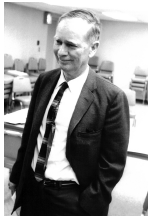
\includegraphics[height=\textheight]{andrews_f_emerson.png} &%
\fontsize{24pt}{24pt}\selectfont \textit{I can promise the ones who wish to stretch their
		minds a bit further that they will not go
		unrewarded.\ldots Modern mathematicians generally
		admit that `the duodecimal system' would be better
		than our present decimal system.\ldots [Dozenal]
		promises to be mathematics' next great step forward
		--- the adoption of an efficient number system.}\par\vskip.5em \fontsize{18pt}{18pt}\selectfont \hbox{\textsc{\vbox{\hangafter=0\hangindent=2em%
	F.
		Emerson Andrews}}}\\%
\end{tabular}%
\end{landscape}%
		\begin{landscape}
		\renewcommand*{\arraystretch}{1.2}
		\vspace{-1em}\centering\monthsty{December 11\e8}\vskip1em
		\noindent
		\begin{tabular}{|%
			>{\daysty\vspace{-.5em}}p{\daywidth}<{\vspace{-.8em}}|%
			>{\daysty\vspace{-.5em}}p{\daywidth}<{\vspace{-.8em}}|%
			>{\daysty\vspace{-.5em}}p{\daywidth}<{\vspace{-.8em}}|%
			>{\daysty\vspace{-.5em}}p{\daywidth}<{\vspace{-.8em}}|%
			>{\daysty\vspace{-.5em}}p{\daywidth}<{\vspace{-.8em}}|%
			>{\daysty\vspace{-.5em}}p{\daywidth}<{\vspace{-.8em}}|%
			>{\daysty\vspace{-.5em}}p{\daywidth}<{\vspace{-.8em}}|}
		\hline
		Sunday & Monday & Tuesday & Wednesday & Thursday%
		& Friday & Saturday \\
		\end{tabular}\vskip-1.4pt

\renewcommand*{\arraystretch}{1.2}
\noindent
\begin{tabular}{|p{\daywidth}|p{\daywidth}|%
p{\daywidth}|p{\daywidth}|p{\daywidth}|p{\daywidth}|%
p{\daywidth}|}
\hline
\multicolumn{6}{|c|}{
\hbox to 6\daywidth{%

	\hfil\hbox to\daywidth{%

		\vbox to.2\dayheight{\vskip2pt%

			\hbox to\daywidth{\hfil\thumbtitsty%

				November\hfil}\vskip2pt%

			\hbox to\daywidth{\hfil%

				\usebox{\monthnegtwo}\hfil}%

		}%

	}%

	\hfil\hbox to\daywidth{%

		\vbox to.2\dayheight{\vskip2pt%

			\hbox to\daywidth{\hfil\thumbtitsty%

				January\hfil}\vskip2pt%

			\hbox to\daywidth{\hfil%

				\usebox{\monthone}\hfil}%

		}%

	}\hfil%

}%

} &
\vtop to\dayheight {\hbox to \linewidth{\hfil\numsty 1\ls}
\rule{0pt}{\dayheight}}\\\hline
\vtop to\dayheight {\hbox to \linewidth{\hfil\numsty 2\ls}
\rule{0pt}{\dayheight}}&\vtop to\dayheight {\hbox to \linewidth{\hfil\numsty 3\ls}
\rule{0pt}{\dayheight}}&\vtop to\dayheight {\hbox to \linewidth{\hfil\numsty 4\ls}
\rule{0pt}{\dayheight}}&\vtop to\dayheight {\hbox to \linewidth{\hfil\numsty 5\ls}
\rule{0pt}{\dayheight}}&\vtop to\dayheight {\hbox to \linewidth{\hfil\numsty 6\ls}
\rule{0pt}{\dayheight}}&\vtop to\dayheight {\hbox to \linewidth{\hfil\numsty 7\ls}
\rule{0pt}{\dayheight}}&\vtop to\dayheight {\hbox to \linewidth{\hfil\numsty 8\ls}
\rule{0pt}{\dayheight}}\\\hline
\vtop to\dayheight {\hbox to \linewidth{\hfil\numsty 9\ls}
\rule{0pt}{\dayheight}}&\vtop to\dayheight {\hbox to \linewidth{\hfil\numsty \x\ls}
\rule{0pt}{\dayheight}}&\vtop to\dayheight {\hbox to \linewidth{\hfil\numsty \e\ls}
\rule{0pt}{\dayheight}}&\vtop to\dayheight {\hbox to \linewidth{\hfil\numsty 10\ls}
\rule{0pt}{\dayheight}}&\vtop to\dayheight {\hbox to \linewidth{\hfil\numsty 11\ls}
\rule{0pt}{\dayheight}}&\vtop to\dayheight {\hbox to \linewidth{\hfil\numsty 12\ls}
\rule{0pt}{\dayheight}}&\vtop to\dayheight {\hbox to \linewidth{\hfil\numsty 13\ls}
\rule{0pt}{\dayheight}}\\\hline
\vtop to\dayheight {\hbox to \linewidth{\hfil\numsty 14\ls}
\rule{0pt}{\dayheight}}&\vtop to\dayheight {\hbox to \linewidth{\hfil\numsty 15\ls}
\rule{0pt}{\dayheight}}&\vtop to\dayheight {\hbox to \linewidth{\hfil\numsty 16\ls}
\rule{0pt}{\dayheight}}&\vtop to\dayheight {\hbox to \linewidth{\hfil\numsty 17\ls}
\rule{0pt}{\dayheight}}&\vtop to\dayheight {\hbox to \linewidth{\hfil\numsty 18\ls}
\rule{0pt}{\dayheight}}&\vtop to\dayheight {\hbox to \linewidth{\hfil\numsty 19\ls}
\rule{0pt}{\dayheight}}&\vtop to\dayheight {\hbox to \linewidth{\hfil\numsty 1\x\ls}
\rule{0pt}{\dayheight}}\\\hline
{\vtop to.3\dayheight {\hbox to \linewidth{\hfil\numsty 1\e\shorts}
}\vfill}\vspace{1.3em}\hbox{\rule{\linewidth}{.4pt}}
{\vtop to.3\dayheight {\hbox to \linewidth{\hfil\numsty 26\shorts}
}}&
{\vtop to.3\dayheight {\hbox to \linewidth{\hfil\numsty 20\shorts}
}\vfill}\vspace{1.3em}\hbox{\rule{\linewidth}{.4pt}}
{\vtop to.3\dayheight {\hbox to \linewidth{\hfil\numsty 27\shorts}
}}&
\vtop to\dayheight {\hbox to \linewidth{\hfil\numsty 21\ls}
\rule{0pt}{\dayheight}}&\vtop to\dayheight {\hbox to \linewidth{\hfil\numsty 22\ls}
\rule{0pt}{\dayheight}}&\vtop to\dayheight {\hbox to \linewidth{\hfil\numsty 23\ls}
\rule{0pt}{\dayheight}}&\vtop to\dayheight {\hbox to \linewidth{\hfil\numsty 24\ls}
\rule{0pt}{\dayheight}}&\vtop to\dayheight {\hbox to \linewidth{\hfil\numsty 25\ls}
\rule{0pt}{\dayheight}}\\\hline\end{tabular}
\end{landscape}
\newpage
\begin{landscape}%
\renewcommand{\tabcolsep}{1em}%
\begin{tabular*}{\textwidth}{>{\hfil}m{.47\linewidth}<{\hfil}m{.47\linewidth}}%

\includegraphics[height=\textheight]{beard_ralph.jpg} &%
\fontsize{24pt}{24pt}\selectfont \textit{Literally, the decimal base is
		unsatis\textsc{factor}y because
		it has \textsc{not enough factors}.\ldots [N]o
		change should be forced, and we urge no mandated
		change.\ldots But people of understanding should
		learn to use duodecimals to facilitate their thinking,
		their computations and their measurings.\ldots In any
		operation, the most advantageous base should be
		used\ldots If this were done, duodecimals would
		progressively earn their way into general
		popularity.}\par\vskip.5em \fontsize{18pt}{18pt}\selectfont \hbox{\textsc{\vbox{\hangafter=0\hangindent=2em%
	Ralph Beard}}}\\%
\end{tabular}%
\end{landscape}%
		\begin{landscape}
		\renewcommand*{\arraystretch}{1.2}
		\vspace{-1em}\centering\monthsty{January 11\e9}\vskip1em
		\noindent
		\begin{tabular}{|%
			>{\daysty\vspace{-.5em}}p{\daywidth}<{\vspace{-.8em}}|%
			>{\daysty\vspace{-.5em}}p{\daywidth}<{\vspace{-.8em}}|%
			>{\daysty\vspace{-.5em}}p{\daywidth}<{\vspace{-.8em}}|%
			>{\daysty\vspace{-.5em}}p{\daywidth}<{\vspace{-.8em}}|%
			>{\daysty\vspace{-.5em}}p{\daywidth}<{\vspace{-.8em}}|%
			>{\daysty\vspace{-.5em}}p{\daywidth}<{\vspace{-.8em}}|%
			>{\daysty\vspace{-.5em}}p{\daywidth}<{\vspace{-.8em}}|}
		\hline
		Sunday & Monday & Tuesday & Wednesday & Thursday%
		& Friday & Saturday \\
		\end{tabular}\vskip-1.4pt

\renewcommand*{\arraystretch}{1.2}
\noindent
\begin{tabular}{|p{\daywidth}|p{\daywidth}|%
p{\daywidth}|p{\daywidth}|p{\daywidth}|p{\daywidth}|%
p{\daywidth}|}
\hline
\multicolumn{2}{|c|}{
\hbox to 2\daywidth{%

	\hfil\hbox to\daywidth{%

		\vbox to.2\dayheight{\vskip2pt%

			\hbox to\daywidth{\hfil\thumbtitsty%

				December\hfil}\vskip2pt%

			\hbox to\daywidth{\hfil%

				\usebox{\monthnegone}\hfil}%

		}%

	}\hfil%

}%

} &
\vtop to\dayheight {\hbox to \linewidth{\hfil\numsty 1\ls}
\rule{0pt}{\dayheight}}&\vtop to\dayheight {\hbox to \linewidth{\hfil\numsty 2\ls}
\rule{0pt}{\dayheight}}&\vtop to\dayheight {\hbox to \linewidth{\hfil\numsty 3\ls}
\rule{0pt}{\dayheight}}&\vtop to\dayheight {\hbox to \linewidth{\hfil\numsty 4\ls}
\rule{0pt}{\dayheight}}&\vtop to\dayheight {\hbox to \linewidth{\hfil\numsty 5\ls}
\rule{0pt}{\dayheight}}\\\hline
\vtop to\dayheight {\hbox to \linewidth{\hfil\numsty 6\ls}
\rule{0pt}{\dayheight}}&\vtop to\dayheight {\hbox to \linewidth{\hfil\numsty 7\ls}
\rule{0pt}{\dayheight}}&\vtop to\dayheight {\hbox to \linewidth{\hfil\numsty 8\ls}
\rule{0pt}{\dayheight}}&\vtop to\dayheight {\hbox to \linewidth{\hfil\numsty 9\ls}
\rule{0pt}{\dayheight}}&\vtop to\dayheight {\hbox to \linewidth{\hfil\numsty \x\ls}
\rule{0pt}{\dayheight}}&\vtop to\dayheight {\hbox to \linewidth{\hfil\numsty \e\ls}
\rule{0pt}{\dayheight}}&\vtop to\dayheight {\hbox to \linewidth{\hfil\numsty 10\ls}
\rule{0pt}{\dayheight}}\\\hline
\vtop to\dayheight {\hbox to \linewidth{\hfil\numsty 11\ls}
\rule{0pt}{\dayheight}}&\vtop to\dayheight {\hbox to \linewidth{\hfil\numsty 12\ls}
\rule{0pt}{\dayheight}}&\vtop to\dayheight {\hbox to \linewidth{\hfil\numsty 13\ls}
\rule{0pt}{\dayheight}}&\vtop to\dayheight {\hbox to \linewidth{\hfil\numsty 14\ls}
\rule{0pt}{\dayheight}}&\vtop to\dayheight {\hbox to \linewidth{\hfil\numsty 15\ls}
\rule{0pt}{\dayheight}}&\vtop to\dayheight {\hbox to \linewidth{\hfil\numsty 16\ls}
\rule{0pt}{\dayheight}}&\vtop to\dayheight {\hbox to \linewidth{\hfil\numsty 17\ls}
\rule{0pt}{\dayheight}}\\\hline
\vtop to\dayheight {\hbox to \linewidth{\hfil\numsty 18\ls}
\rule{0pt}{\dayheight}}&\vtop to\dayheight {\hbox to \linewidth{\hfil\numsty 19\ls}
\rule{0pt}{\dayheight}}&\vtop to\dayheight {\hbox to \linewidth{\hfil\numsty 1\x\ls}
\rule{0pt}{\dayheight}}&\vtop to\dayheight {\hbox to \linewidth{\hfil\numsty 1\e\ls}
\rule{0pt}{\dayheight}}&\vtop to\dayheight {\hbox to \linewidth{\hfil\numsty 20\ls}
\rule{0pt}{\dayheight}}&\vtop to\dayheight {\hbox to \linewidth{\hfil\numsty 21\ls}
\rule{0pt}{\dayheight}}&\vtop to\dayheight {\hbox to \linewidth{\hfil\numsty 22\ls}
\rule{0pt}{\dayheight}}\\\hline
\vtop to\dayheight {\hbox to \linewidth{\hfil\numsty 23\ls}
\rule{0pt}{\dayheight}}&\vtop to\dayheight {\hbox to \linewidth{\hfil\numsty 24\ls}
\rule{0pt}{\dayheight}}&\vtop to\dayheight {\hbox to \linewidth{\hfil\numsty 25\ls}
\rule{0pt}{\dayheight}}&\vtop to\dayheight {\hbox to \linewidth{\hfil\numsty 26\ls}
\rule{0pt}{\dayheight}}&\vtop to\dayheight {\hbox to \linewidth{\hfil\numsty 27\ls}
\rule{0pt}{\dayheight}}&\multicolumn{2}{c|}{
\hbox to 2\daywidth{%

	\hfil\hbox to\daywidth{%

		\vbox to.2\dayheight{\vskip2pt%

			\hbox to\daywidth{\hfil\thumbtitsty%

				February\hfil}\vskip2pt%

			\hbox to\daywidth{\hfil%

				\usebox{\monthtwo}\hfil}%

		}%

	}\hfil%

}%

} &
\hline\end{tabular}
\end{landscape}
\newpage
\begin{landscape}%
\renewcommand{\tabcolsep}{1em}%
\vspace*{\stretch{1}}%
\begin{tabular*}{\textwidth}{>{\hfil}m{.47\linewidth}<{\hfil}m{.47\linewidth}}%

\includegraphics[height=0.6\textheight]{logo_shapes_dozenal.mps} &%
\fontsize{24pt}{24pt}\selectfont \textit{The offspring of the dozen serve us well.  Five of
		the six possible figures are convex polygons and four
		of these are essential to engineering and
		mathematics.\ldots Need we search any further for a
		rational, serviceable number-base?  Can there possibly
		be a better?}\par\vskip.5em \fontsize{18pt}{18pt}\selectfont \hbox{\textsc{\vbox{\hangafter=0\hangindent=2em%
	Troy, DSGB}}}\\%
\end{tabular}%
\vspace*{\stretch{1}}%
\end{landscape}%
		\begin{landscape}
		\renewcommand*{\arraystretch}{1.2}
		\vspace{-1em}\centering\monthsty{February 11\e9}\vskip1em
		\noindent
		\begin{tabular}{|%
			>{\daysty\vspace{-.5em}}p{\daywidth}<{\vspace{-.8em}}|%
			>{\daysty\vspace{-.5em}}p{\daywidth}<{\vspace{-.8em}}|%
			>{\daysty\vspace{-.5em}}p{\daywidth}<{\vspace{-.8em}}|%
			>{\daysty\vspace{-.5em}}p{\daywidth}<{\vspace{-.8em}}|%
			>{\daysty\vspace{-.5em}}p{\daywidth}<{\vspace{-.8em}}|%
			>{\daysty\vspace{-.5em}}p{\daywidth}<{\vspace{-.8em}}|%
			>{\daysty\vspace{-.5em}}p{\daywidth}<{\vspace{-.8em}}|}
		\hline
		Sunday & Monday & Tuesday & Wednesday & Thursday%
		& Friday & Saturday \\
		\end{tabular}\vskip-1.4pt

\renewcommand*{\arraystretch}{1.2}
\noindent
\begin{tabular}{|p{\daywidth}|p{\daywidth}|%
p{\daywidth}|p{\daywidth}|p{\daywidth}|p{\daywidth}|%
p{\daywidth}|}
\hline
\multicolumn{5}{|c|}{
\hbox to 5\daywidth{%

	\hfil\hbox to\daywidth{%

		\vbox to.2\dayheight{\vskip2pt%

			\hbox to\daywidth{\hfil\thumbtitsty%

				January\hfil}\vskip2pt%

			\hbox to\daywidth{\hfil%

				\usebox{\monthone}\hfil}%

		}%

	}%

	\hfil\hbox to\daywidth{%

		\vbox to.2\dayheight{\vskip2pt%

			\hbox to\daywidth{\hfil\thumbtitsty%

				March\hfil}\vskip2pt%

			\hbox to\daywidth{\hfil%

				\usebox{\monththree}\hfil}%

		}%

	}\hfil%

}%

} &
\vtop to\dayheight {\hbox to \linewidth{\hfil\numsty 1\ls}
\rule{0pt}{\dayheight}}&\vtop to\dayheight {\hbox to \linewidth{\hfil\numsty 2\ls}
\rule{0pt}{\dayheight}}\\\hline
\vtop to\dayheight {\hbox to \linewidth{\hfil\numsty 3\ls}
\rule{0pt}{\dayheight}}&\vtop to\dayheight {\hbox to \linewidth{\hfil\numsty 4\ls}
\rule{0pt}{\dayheight}}&\vtop to\dayheight {\hbox to \linewidth{\hfil\numsty 5\ls}
\rule{0pt}{\dayheight}}&\vtop to\dayheight {\hbox to \linewidth{\hfil\numsty 6\ls}
\rule{0pt}{\dayheight}}&\vtop to\dayheight {\hbox to \linewidth{\hfil\numsty 7\ls}
\rule{0pt}{\dayheight}}&\vtop to\dayheight {\hbox to \linewidth{\hfil\numsty 8\ls}
\rule{0pt}{\dayheight}}&\vtop to\dayheight {\hbox to \linewidth{\hfil\numsty 9\ls}
\rule{0pt}{\dayheight}}\\\hline
\vtop to\dayheight {\hbox to \linewidth{\hfil\numsty \x\ls}
\rule{0pt}{\dayheight}}&\vtop to\dayheight {\hbox to \linewidth{\hfil\numsty \e\ls}
\rule{0pt}{\dayheight}}&\vtop to\dayheight {\hbox to \linewidth{\hfil\numsty 10\ls}
\rule{0pt}{\dayheight}}&\vtop to\dayheight {\hbox to \linewidth{\hfil\numsty 11\ls}
\rule{0pt}{\dayheight}}&\vtop to\dayheight {\hbox to \linewidth{\hfil\numsty 12\ls}
\rule{0pt}{\dayheight}}&\vtop to\dayheight {\hbox to \linewidth{\hfil\numsty 13\ls}
\rule{0pt}{\dayheight}}&\vtop to\dayheight {\hbox to \linewidth{\hfil\numsty 14\ls}
\rule{0pt}{\dayheight}}\\\hline
\vtop to\dayheight {\hbox to \linewidth{\hfil\numsty 15\ls}
\rule{0pt}{\dayheight}}&\vtop to\dayheight {\hbox to \linewidth{\hfil\numsty 16\ls}
\rule{0pt}{\dayheight}}&\vtop to\dayheight {\hbox to \linewidth{\hfil\numsty 17\ls}
\rule{0pt}{\dayheight}}&\vtop to\dayheight {\hbox to \linewidth{\hfil\numsty 18\ls}
\rule{0pt}{\dayheight}}&\vtop to\dayheight {\hbox to \linewidth{\hfil\numsty 19\ls}
\rule{0pt}{\dayheight}}&\vtop to\dayheight {\hbox to \linewidth{\hfil\numsty 1\x\ls}
\rule{0pt}{\dayheight}}&\vtop to\dayheight {\hbox to \linewidth{\hfil\numsty 1\e\ls}
\rule{0pt}{\dayheight}}\\\hline
\vtop to\dayheight {\hbox to \linewidth{\hfil\numsty 20\ls}
\rule{0pt}{\dayheight}}&\vtop to\dayheight {\hbox to \linewidth{\hfil\numsty 21\ls}
\rule{0pt}{\dayheight}}&\vtop to\dayheight {\hbox to \linewidth{\hfil\numsty 22\ls}
\rule{0pt}{\dayheight}}&\vtop to\dayheight {\hbox to \linewidth{\hfil\numsty 23\ls}
\rule{0pt}{\dayheight}}&\vtop to\dayheight {\hbox to \linewidth{\hfil\numsty 24\ls}
\rule{0pt}{\dayheight}}&\multicolumn{2}{c|}{
\hbox to 2\daywidth{%

	\hfil\hbox to\daywidth{%

		\vbox to.2\dayheight{\vskip2pt%

			\hbox to\daywidth{\hfil\thumbtitsty%

				March\hfil}\vskip2pt%

			\hbox to\daywidth{\hfil%

				\usebox{\monththree}\hfil}%

		}%

	}\hfil%

}%

} &
\hline\end{tabular}
\end{landscape}
\newpage
\begin{landscape}%
\renewcommand{\tabcolsep}{1em}%
\vspace*{\stretch{1}}%
\begin{tabular*}{\textwidth}{>{\hfil}m{.47\linewidth}<{\hfil}m{.47\linewidth}}%
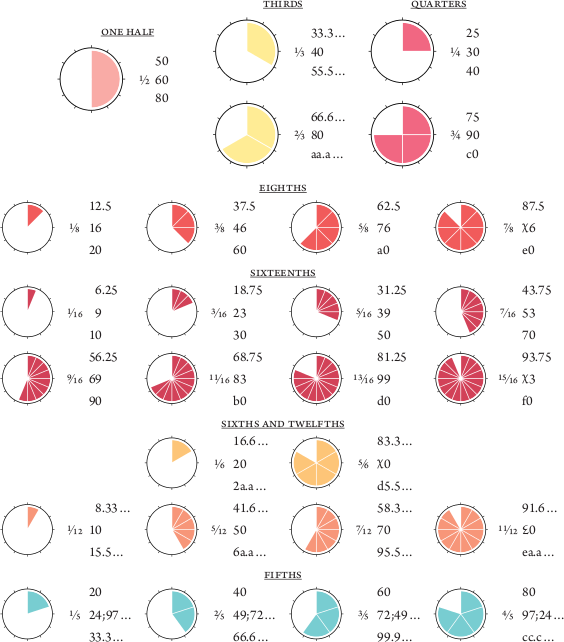
\includegraphics[height=0.75\textheight]{dozenal_fractions.png} &%
\fontsize{24pt}{24pt}\selectfont \textit{[T]welve is a highly
		divisible yet compact number; it has more divisors
		than ten.  This facilitates learning and using
		arithmetic, and simplifies the natural fractions.}\par\vskip.5em \fontsize{18pt}{18pt}\selectfont \hbox{\textsc{\vbox{\hangafter=0\hangindent=2em%
	Michael deVlieger}}}\\%
\end{tabular}%
\vspace*{\stretch{1}}%
\end{landscape}%
		\begin{landscape}
		\renewcommand*{\arraystretch}{1.2}
		\vspace{-1em}\centering\monthsty{March 11\e9}\vskip1em
		\noindent
		\begin{tabular}{|%
			>{\daysty\vspace{-.5em}}p{\daywidth}<{\vspace{-.8em}}|%
			>{\daysty\vspace{-.5em}}p{\daywidth}<{\vspace{-.8em}}|%
			>{\daysty\vspace{-.5em}}p{\daywidth}<{\vspace{-.8em}}|%
			>{\daysty\vspace{-.5em}}p{\daywidth}<{\vspace{-.8em}}|%
			>{\daysty\vspace{-.5em}}p{\daywidth}<{\vspace{-.8em}}|%
			>{\daysty\vspace{-.5em}}p{\daywidth}<{\vspace{-.8em}}|%
			>{\daysty\vspace{-.5em}}p{\daywidth}<{\vspace{-.8em}}|}
		\hline
		Sunday & Monday & Tuesday & Wednesday & Thursday%
		& Friday & Saturday \\
		\end{tabular}\vskip-1.4pt

\renewcommand*{\arraystretch}{1.2}
\noindent
\begin{tabular}{|p{\daywidth}|p{\daywidth}|%
p{\daywidth}|p{\daywidth}|p{\daywidth}|p{\daywidth}|%
p{\daywidth}|}
\hline
\multicolumn{5}{|c|}{
\hbox to 5\daywidth{%

	\hfil\hbox to\daywidth{%

		\vbox to.2\dayheight{\vskip2pt%

			\hbox to\daywidth{\hfil\thumbtitsty%

				February\hfil}\vskip2pt%

			\hbox to\daywidth{\hfil%

				\usebox{\monthtwo}\hfil}%

		}%

	}%

	\hfil\hbox to\daywidth{%

		\vbox to.2\dayheight{\vskip2pt%

			\hbox to\daywidth{\hfil\thumbtitsty%

				April\hfil}\vskip2pt%

			\hbox to\daywidth{\hfil%

				\usebox{\monthfour}\hfil}%

		}%

	}\hfil%

}%

} &
\vtop to\dayheight {\hbox to \linewidth{\hfil\numsty 1\ls}
\rule{0pt}{\dayheight}}&\vtop to\dayheight {\hbox to \linewidth{\hfil\numsty 2\ls}
\rule{0pt}{\dayheight}}\\\hline
\vtop to\dayheight {\hbox to \linewidth{\hfil\numsty 3\ls}
\rule{0pt}{\dayheight}}&\vtop to\dayheight {\hbox to \linewidth{\hfil\numsty 4\ls}
\rule{0pt}{\dayheight}}&\vtop to\dayheight {\hbox to \linewidth{\hfil\numsty 5\ls}
\rule{0pt}{\dayheight}}&\vtop to\dayheight {\hbox to \linewidth{\hfil\numsty 6\ls}
\rule{0pt}{\dayheight}}&\vtop to\dayheight {\hbox to \linewidth{\hfil\numsty 7\ls}
\rule{0pt}{\dayheight}}&\vtop to\dayheight {\hbox to \linewidth{\hfil\numsty 8\ls}
\rule{0pt}{\dayheight}}&\vtop to\dayheight {\hbox to \linewidth{\hfil\numsty 9\ls}
\rule{0pt}{\dayheight}}\\\hline
\vtop to\dayheight {\hbox to \linewidth{\hfil\numsty \x\ls}
\rule{0pt}{\dayheight}}&\vtop to\dayheight {\hbox to \linewidth{\hfil\numsty \e\ls}
\rule{0pt}{\dayheight}}&\vtop to\dayheight {\hbox to \linewidth{\hfil\numsty 10\ls}
\rule{0pt}{\dayheight}}&\vtop to\dayheight {\hbox to \linewidth{\hfil\numsty 11\ls}
\rule{0pt}{\dayheight}}&\vtop to\dayheight {\hbox to \linewidth{\hfil\numsty 12\ls}
\rule{0pt}{\dayheight}}&\vtop to\dayheight {\hbox to \linewidth{\hfil\numsty 13\ls}
\rule{0pt}{\dayheight}}&\vtop to\dayheight {\hbox to \linewidth{\hfil\numsty 14\ls}
\rule{0pt}{\dayheight}}\\\hline
\vtop to\dayheight {\hbox to \linewidth{\hfil\numsty 15\ls}
\rule{0pt}{\dayheight}}&\vtop to\dayheight {\hbox to \linewidth{\hfil\numsty 16\ls}
\rule{0pt}{\dayheight}}&\vtop to\dayheight {\hbox to \linewidth{\hfil\numsty 17\ls}
\rule{0pt}{\dayheight}}&\vtop to\dayheight {\hbox to \linewidth{\hfil\numsty 18\ls}
\rule{0pt}{\dayheight}}&\vtop to\dayheight {\hbox to \linewidth{\hfil\numsty 19\ls}
\rule{0pt}{\dayheight}}&\vtop to\dayheight {\hbox to \linewidth{\hfil\numsty 1\x\ls}
\rule{0pt}{\dayheight}}&\vtop to\dayheight {\hbox to \linewidth{\hfil\numsty 1\e\ls}
\rule{0pt}{\dayheight}}\\\hline
{\vtop to.3\dayheight {\hbox to \linewidth{\hfil\numsty 20\shorts}
}\vfill}\vspace{1.3em}\hbox{\rule{\linewidth}{.4pt}}
{\vtop to.3\dayheight {\hbox to \linewidth{\hfil\numsty 27\shorts}
}}&
\vtop to\dayheight {\hbox to \linewidth{\hfil\numsty 21\ls}
\rule{0pt}{\dayheight}}&\vtop to\dayheight {\hbox to \linewidth{\hfil\numsty 22\ls}
\rule{0pt}{\dayheight}}&\vtop to\dayheight {\hbox to \linewidth{\hfil\numsty 23\ls}
\rule{0pt}{\dayheight}}&\vtop to\dayheight {\hbox to \linewidth{\hfil\numsty 24\ls}
\rule{0pt}{\dayheight}}&\vtop to\dayheight {\hbox to \linewidth{\hfil\numsty 25\ls}
\rule{0pt}{\dayheight}}&\vtop to\dayheight {\hbox to \linewidth{\hfil\numsty 26\ls}
\rule{0pt}{\dayheight}}\\\hline\end{tabular}
\end{landscape}
\newpage
\begin{landscape}%
\renewcommand{\tabcolsep}{1em}%
\vspace*{\stretch{1}}%
\begin{tabular*}{\textwidth}{>{\hfil}m{.47\linewidth}<{\hfil}m{.47\linewidth}}%
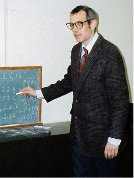
\includegraphics[height=0.8\textheight]{schiffman_jay.jpg} &%
\fontsize{24pt}{24pt}\selectfont \textit{One dozen is the
		\emph{initial abundant number}.\ldots The dozen is
		\emph{hypercomposite}.\ldots The dozen represents
		the first number which is \emph{neither a Converse
		Lagrange Theorem group} (CLT) \emph{nor
		supersolvable}.\ldots One dozen is the first natural
		number having a \emph{perfect number of divisors}
		(six).}\par\vskip.5em \fontsize{18pt}{18pt}\selectfont \hbox{\textsc{\vbox{\hangafter=0\hangindent=2em%
	Prof. Jay Schiffman}}}\\%
\end{tabular}%
\vspace*{\stretch{1}}%
\end{landscape}%
		\begin{landscape}
		\renewcommand*{\arraystretch}{1.2}
		\vspace{-1em}\centering\monthsty{April 11\e9}\vskip1em
		\noindent
		\begin{tabular}{|%
			>{\daysty\vspace{-.5em}}p{\daywidth}<{\vspace{-.8em}}|%
			>{\daysty\vspace{-.5em}}p{\daywidth}<{\vspace{-.8em}}|%
			>{\daysty\vspace{-.5em}}p{\daywidth}<{\vspace{-.8em}}|%
			>{\daysty\vspace{-.5em}}p{\daywidth}<{\vspace{-.8em}}|%
			>{\daysty\vspace{-.5em}}p{\daywidth}<{\vspace{-.8em}}|%
			>{\daysty\vspace{-.5em}}p{\daywidth}<{\vspace{-.8em}}|%
			>{\daysty\vspace{-.5em}}p{\daywidth}<{\vspace{-.8em}}|}
		\hline
		Sunday & Monday & Tuesday & Wednesday & Thursday%
		& Friday & Saturday \\
		\end{tabular}\vskip-1.4pt

\renewcommand*{\arraystretch}{1.2}
\noindent
\begin{tabular}{|p{\daywidth}|p{\daywidth}|%
p{\daywidth}|p{\daywidth}|p{\daywidth}|p{\daywidth}|%
p{\daywidth}|}
\hline
\multicolumn{1}{|c|}{
\hbox to 1\daywidth{%

	\hfil\hbox to\daywidth{%

		\vbox to.2\dayheight{\vskip2pt%

			\hbox to\daywidth{\hfil\thumbtitsty%

				March\hfil}\vskip2pt%

			\hbox to\daywidth{\hfil%

				\usebox{\monththree}\hfil}%

		}%

	}\hfil%

}%

} &
\vtop to\dayheight {\hbox to \linewidth{\hfil\numsty 1\ls}
\rule{0pt}{\dayheight}}&\vtop to\dayheight {\hbox to \linewidth{\hfil\numsty 2\ls}
\rule{0pt}{\dayheight}}&\vtop to\dayheight {\hbox to \linewidth{\hfil\numsty 3\ls}
\rule{0pt}{\dayheight}}&\vtop to\dayheight {\hbox to \linewidth{\hfil\numsty 4\ls}
\rule{0pt}{\dayheight}}&\vtop to\dayheight {\hbox to \linewidth{\hfil\numsty 5\ls}
\rule{0pt}{\dayheight}}&\vtop to\dayheight {\hbox to \linewidth{\hfil\numsty 6\ls}
\rule{0pt}{\dayheight}}\\\hline
\vtop to\dayheight {\hbox to \linewidth{\hfil\numsty 7\ls}
\rule{0pt}{\dayheight}}&\vtop to\dayheight {\hbox to \linewidth{\hfil\numsty 8\ls}
\rule{0pt}{\dayheight}}&\vtop to\dayheight {\hbox to \linewidth{\hfil\numsty 9\ls}
\rule{0pt}{\dayheight}}&\vtop to\dayheight {\hbox to \linewidth{\hfil\numsty \x\ls}
\rule{0pt}{\dayheight}}&\vtop to\dayheight {\hbox to \linewidth{\hfil\numsty \e\ls}
\rule{0pt}{\dayheight}}&\vtop to\dayheight {\hbox to \linewidth{\hfil\numsty 10\ls}
\rule{0pt}{\dayheight}}&\vtop to\dayheight {\hbox to \linewidth{\hfil\numsty 11\ls}
\rule{0pt}{\dayheight}}\\\hline
\vtop to\dayheight {\hbox to \linewidth{\hfil\numsty 12\ls}
\rule{0pt}{\dayheight}}&\vtop to\dayheight {\hbox to \linewidth{\hfil\numsty 13\ls}
\rule{0pt}{\dayheight}}&\vtop to\dayheight {\hbox to \linewidth{\hfil\numsty 14\ls}
\rule{0pt}{\dayheight}}&\vtop to\dayheight {\hbox to \linewidth{\hfil\numsty 15\ls}
\rule{0pt}{\dayheight}}&\vtop to\dayheight {\hbox to \linewidth{\hfil\numsty 16\ls}
\rule{0pt}{\dayheight}}&\vtop to\dayheight {\hbox to \linewidth{\hfil\numsty 17\ls}
\rule{0pt}{\dayheight}}&\vtop to\dayheight {\hbox to \linewidth{\hfil\numsty 18\ls}
\rule{0pt}{\dayheight}}\\\hline
\vtop to\dayheight {\hbox to \linewidth{\hfil\numsty 19\ls}
\rule{0pt}{\dayheight}}&\vtop to\dayheight {\hbox to \linewidth{\hfil\numsty 1\x\ls}
\rule{0pt}{\dayheight}}&\vtop to\dayheight {\hbox to \linewidth{\hfil\numsty 1\e\ls}
\rule{0pt}{\dayheight}}&\vtop to\dayheight {\hbox to \linewidth{\hfil\numsty 20\ls}
\rule{0pt}{\dayheight}}&\vtop to\dayheight {\hbox to \linewidth{\hfil\numsty 21\ls}
\rule{0pt}{\dayheight}}&\vtop to\dayheight {\hbox to \linewidth{\hfil\numsty 22\ls}
\rule{0pt}{\dayheight}}&\vtop to\dayheight {\hbox to \linewidth{\hfil\numsty 23\ls}
\rule{0pt}{\dayheight}}\\\hline
\vtop to\dayheight {\hbox to \linewidth{\hfil\numsty 24\ls}
\rule{0pt}{\dayheight}}&\vtop to\dayheight {\hbox to \linewidth{\hfil\numsty 25\ls}
\rule{0pt}{\dayheight}}&\vtop to\dayheight {\hbox to \linewidth{\hfil\numsty 26\ls}
\rule{0pt}{\dayheight}}&\multicolumn{4}{c|}{
\hbox to 4\daywidth{%

	\hfil\hbox to\daywidth{%

		\vbox to.2\dayheight{\vskip2pt%

			\hbox to\daywidth{\hfil\thumbtitsty%

				March\hfil}\vskip2pt%

			\hbox to\daywidth{\hfil%

				\usebox{\monththree}\hfil}%

		}%

	}%

	\hfil\hbox to\daywidth{%

		\vbox to.2\dayheight{\vskip2pt%

			\hbox to\daywidth{\hfil\thumbtitsty%

				May\hfil}\vskip2pt%

			\hbox to\daywidth{\hfil%

				\usebox{\monthfive}\hfil}%

		}%

	}\hfil%

}%

} &
\hline\end{tabular}
\end{landscape}
\newpage
\begin{landscape}%
\renewcommand{\tabcolsep}{1em}%
\vspace*{\stretch{1}}%
\begin{tabular*}{\textwidth}{>{\hfil}m{.47\linewidth}<{\hfil}m{.47\linewidth}}%
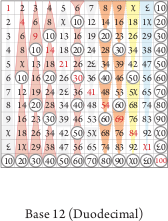
\includegraphics[height=0.8\textheight]{dozenal_times_tables.png} &%
\fontsize{24pt}{24pt}\selectfont \textit{Because twelve
		has six divisors, with the smallest four consecutive,
		it presents a multiplication table featuring brief
		patterns in the product lines of many numbers.\ldots
		[U]sers of duodecimal enjoy two other divisor product
		lines in the multiplication table.}\par\vskip.5em \fontsize{18pt}{18pt}\selectfont \hbox{\textsc{\vbox{\hangafter=0\hangindent=2em%
	Michael
		deVlieger}}}\\%
\end{tabular}%
\vspace*{\stretch{1}}%
\end{landscape}%
		\begin{landscape}
		\renewcommand*{\arraystretch}{1.2}
		\vspace{-1em}\centering\monthsty{May 11\e9}\vskip1em
		\noindent
		\begin{tabular}{|%
			>{\daysty\vspace{-.5em}}p{\daywidth}<{\vspace{-.8em}}|%
			>{\daysty\vspace{-.5em}}p{\daywidth}<{\vspace{-.8em}}|%
			>{\daysty\vspace{-.5em}}p{\daywidth}<{\vspace{-.8em}}|%
			>{\daysty\vspace{-.5em}}p{\daywidth}<{\vspace{-.8em}}|%
			>{\daysty\vspace{-.5em}}p{\daywidth}<{\vspace{-.8em}}|%
			>{\daysty\vspace{-.5em}}p{\daywidth}<{\vspace{-.8em}}|%
			>{\daysty\vspace{-.5em}}p{\daywidth}<{\vspace{-.8em}}|}
		\hline
		Sunday & Monday & Tuesday & Wednesday & Thursday%
		& Friday & Saturday \\
		\end{tabular}\vskip-1.4pt

\renewcommand*{\arraystretch}{1.2}
\noindent
\begin{tabular}{|p{\daywidth}|p{\daywidth}|%
p{\daywidth}|p{\daywidth}|p{\daywidth}|p{\daywidth}|%
p{\daywidth}|}
\hline
\multicolumn{3}{|c|}{
\hbox to 3\daywidth{%

	\hfil\hbox to\daywidth{%

		\vbox to.2\dayheight{\vskip2pt%

			\hbox to\daywidth{\hfil\thumbtitsty%

				April\hfil}\vskip2pt%

			\hbox to\daywidth{\hfil%

				\usebox{\monthfour}\hfil}%

		}%

	}%

	\hfil\hbox to\daywidth{%

		\vbox to.2\dayheight{\vskip2pt%

			\hbox to\daywidth{\hfil\thumbtitsty%

				June\hfil}\vskip2pt%

			\hbox to\daywidth{\hfil%

				\usebox{\monthsix}\hfil}%

		}%

	}\hfil%

}%

} &
\vtop to\dayheight {\hbox to \linewidth{\hfil\numsty 1\ls}
\rule{0pt}{\dayheight}}&\vtop to\dayheight {\hbox to \linewidth{\hfil\numsty 2\ls}
\rule{0pt}{\dayheight}}&\vtop to\dayheight {\hbox to \linewidth{\hfil\numsty 3\ls}
\rule{0pt}{\dayheight}}&\vtop to\dayheight {\hbox to \linewidth{\hfil\numsty 4\ls}
\rule{0pt}{\dayheight}}\\\hline
\vtop to\dayheight {\hbox to \linewidth{\hfil\numsty 5\ls}
\rule{0pt}{\dayheight}}&\vtop to\dayheight {\hbox to \linewidth{\hfil\numsty 6\ls}
\rule{0pt}{\dayheight}}&\vtop to\dayheight {\hbox to \linewidth{\hfil\numsty 7\ls}
\rule{0pt}{\dayheight}}&\vtop to\dayheight {\hbox to \linewidth{\hfil\numsty 8\ls}
\rule{0pt}{\dayheight}}&\vtop to\dayheight {\hbox to \linewidth{\hfil\numsty 9\ls}
\rule{0pt}{\dayheight}}&\vtop to\dayheight {\hbox to \linewidth{\hfil\numsty \x\ls}
\rule{0pt}{\dayheight}}&\vtop to\dayheight {\hbox to \linewidth{\hfil\numsty \e\ls}
\rule{0pt}{\dayheight}}\\\hline
\vtop to\dayheight {\hbox to \linewidth{\hfil\numsty 10\ls}
\rule{0pt}{\dayheight}}&\vtop to\dayheight {\hbox to \linewidth{\hfil\numsty 11\ls}
\rule{0pt}{\dayheight}}&\vtop to\dayheight {\hbox to \linewidth{\hfil\numsty 12\ls}
\rule{0pt}{\dayheight}}&\vtop to\dayheight {\hbox to \linewidth{\hfil\numsty 13\ls}
\rule{0pt}{\dayheight}}&\vtop to\dayheight {\hbox to \linewidth{\hfil\numsty 14\ls}
\rule{0pt}{\dayheight}}&\vtop to\dayheight {\hbox to \linewidth{\hfil\numsty 15\ls}
\rule{0pt}{\dayheight}}&\vtop to\dayheight {\hbox to \linewidth{\hfil\numsty 16\ls}
\rule{0pt}{\dayheight}}\\\hline
\vtop to\dayheight {\hbox to \linewidth{\hfil\numsty 17\ls}
\rule{0pt}{\dayheight}}&\vtop to\dayheight {\hbox to \linewidth{\hfil\numsty 18\ls}
\rule{0pt}{\dayheight}}&\vtop to\dayheight {\hbox to \linewidth{\hfil\numsty 19\ls}
\rule{0pt}{\dayheight}}&\vtop to\dayheight {\hbox to \linewidth{\hfil\numsty 1\x\ls}
\rule{0pt}{\dayheight}}&\vtop to\dayheight {\hbox to \linewidth{\hfil\numsty 1\e\ls}
\rule{0pt}{\dayheight}}&\vtop to\dayheight {\hbox to \linewidth{\hfil\numsty 20\ls}
\rule{0pt}{\dayheight}}&\vtop to\dayheight {\hbox to \linewidth{\hfil\numsty 21\ls}
\rule{0pt}{\dayheight}}\\\hline
\vtop to\dayheight {\hbox to \linewidth{\hfil\numsty 22\ls}
\rule{0pt}{\dayheight}}&\vtop to\dayheight {\hbox to \linewidth{\hfil\numsty 23\ls}
\rule{0pt}{\dayheight}}&\vtop to\dayheight {\hbox to \linewidth{\hfil\numsty 24\ls}
\rule{0pt}{\dayheight}}&\vtop to\dayheight {\hbox to \linewidth{\hfil\numsty 25\ls}
\rule{0pt}{\dayheight}}&\vtop to\dayheight {\hbox to \linewidth{\hfil\numsty 26\ls}
\rule{0pt}{\dayheight}}&\vtop to\dayheight {\hbox to \linewidth{\hfil\numsty 27\ls}
\rule{0pt}{\dayheight}}&\multicolumn{1}{c|}{
\hbox to 1\daywidth{%

	\hfil\hbox to\daywidth{%

		\vbox to.2\dayheight{\vskip2pt%

			\hbox to\daywidth{\hfil\thumbtitsty%

				June\hfil}\vskip2pt%

			\hbox to\daywidth{\hfil%

				\usebox{\monthsix}\hfil}%

		}%

	}\hfil%

}%

} &
\hline\end{tabular}
\end{landscape}
\newpage
\begin{landscape}%
\renewcommand{\tabcolsep}{1em}%
\vspace*{\stretch{1}}%
\begin{tabular*}{\textwidth}{>{\hfil}m{.47\linewidth}<{\hfil}m{.47\linewidth}}%
\includegraphics[height=0.4\textheight,angle=90]{keyb_doz.mps} &%
\fontsize{24pt}{24pt}\selectfont \textit{\emph{There are twelve
		equal notes in an octave}.\ldots [They are]
		logarithms to base two.  Expressed in dozenal
		numeration they form a unique system for handling
		ratios, with simplicities not found in any other
		system.  The music keyboard was caused to have twelve
		semitones to the octave by this.}\par\vskip.5em \fontsize{18pt}{18pt}\selectfont \hbox{\textsc{\vbox{\hangafter=0\hangindent=2em%
	Tom
		Pendlebury}}}\\%
\end{tabular}%
\vspace*{\stretch{1}}%
\end{landscape}%
		\begin{landscape}
		\renewcommand*{\arraystretch}{1.2}
		\vspace{-1em}\centering\monthsty{June 11\e9}\vskip1em
		\noindent
		\begin{tabular}{|%
			>{\daysty\vspace{-.5em}}p{\daywidth}<{\vspace{-.8em}}|%
			>{\daysty\vspace{-.5em}}p{\daywidth}<{\vspace{-.8em}}|%
			>{\daysty\vspace{-.5em}}p{\daywidth}<{\vspace{-.8em}}|%
			>{\daysty\vspace{-.5em}}p{\daywidth}<{\vspace{-.8em}}|%
			>{\daysty\vspace{-.5em}}p{\daywidth}<{\vspace{-.8em}}|%
			>{\daysty\vspace{-.5em}}p{\daywidth}<{\vspace{-.8em}}|%
			>{\daysty\vspace{-.5em}}p{\daywidth}<{\vspace{-.8em}}|}
		\hline
		Sunday & Monday & Tuesday & Wednesday & Thursday%
		& Friday & Saturday \\
		\end{tabular}\vskip-1.4pt

\renewcommand*{\arraystretch}{1.2}
\noindent
\begin{tabular}{|p{\daywidth}|p{\daywidth}|%
p{\daywidth}|p{\daywidth}|p{\daywidth}|p{\daywidth}|%
p{\daywidth}|}
\hline
\multicolumn{6}{|c|}{
\hbox to 6\daywidth{%

	\hfil\hbox to\daywidth{%

		\vbox to.2\dayheight{\vskip2pt%

			\hbox to\daywidth{\hfil\thumbtitsty%

				May\hfil}\vskip2pt%

			\hbox to\daywidth{\hfil%

				\usebox{\monthfive}\hfil}%

		}%

	}%

	\hfil\hbox to\daywidth{%

		\vbox to.2\dayheight{\vskip2pt%

			\hbox to\daywidth{\hfil\thumbtitsty%

				July\hfil}\vskip2pt%

			\hbox to\daywidth{\hfil%

				\usebox{\monthseven}\hfil}%

		}%

	}\hfil%

}%

} &
\vtop to\dayheight {\hbox to \linewidth{\hfil\numsty 1\ls}
\rule{0pt}{\dayheight}}\\\hline
\vtop to\dayheight {\hbox to \linewidth{\hfil\numsty 2\ls}
\rule{0pt}{\dayheight}}&\vtop to\dayheight {\hbox to \linewidth{\hfil\numsty 3\ls}
\rule{0pt}{\dayheight}}&\vtop to\dayheight {\hbox to \linewidth{\hfil\numsty 4\ls}
\rule{0pt}{\dayheight}}&\vtop to\dayheight {\hbox to \linewidth{\hfil\numsty 5\ls}
\rule{0pt}{\dayheight}}&\vtop to\dayheight {\hbox to \linewidth{\hfil\numsty 6\ls}
\rule{0pt}{\dayheight}}&\vtop to\dayheight {\hbox to \linewidth{\hfil\numsty 7\ls}
\rule{0pt}{\dayheight}}&\vtop to\dayheight {\hbox to \linewidth{\hfil\numsty 8\ls}
\rule{0pt}{\dayheight}}\\\hline
\vtop to\dayheight {\hbox to \linewidth{\hfil\numsty 9\ls}
\rule{0pt}{\dayheight}}&\vtop to\dayheight {\hbox to \linewidth{\hfil\numsty \x\ls}
\rule{0pt}{\dayheight}}&\vtop to\dayheight {\hbox to \linewidth{\hfil\numsty \e\ls}
\rule{0pt}{\dayheight}}&\vtop to\dayheight {\hbox to \linewidth{\hfil\numsty 10\ls}
\rule{0pt}{\dayheight}}&\vtop to\dayheight {\hbox to \linewidth{\hfil\numsty 11\ls}
\rule{0pt}{\dayheight}}&\vtop to\dayheight {\hbox to \linewidth{\hfil\numsty 12\ls}
\rule{0pt}{\dayheight}}&\vtop to\dayheight {\hbox to \linewidth{\hfil\numsty 13\ls}
\rule{0pt}{\dayheight}}\\\hline
\vtop to\dayheight {\hbox to \linewidth{\hfil\numsty 14\ls}
\rule{0pt}{\dayheight}}&\vtop to\dayheight {\hbox to \linewidth{\hfil\numsty 15\ls}
\rule{0pt}{\dayheight}}&\vtop to\dayheight {\hbox to \linewidth{\hfil\numsty 16\ls}
\rule{0pt}{\dayheight}}&\vtop to\dayheight {\hbox to \linewidth{\hfil\numsty 17\ls}
\rule{0pt}{\dayheight}}&\vtop to\dayheight {\hbox to \linewidth{\hfil\numsty 18\ls}
\rule{0pt}{\dayheight}}&\vtop to\dayheight {\hbox to \linewidth{\hfil\numsty 19\ls}
\rule{0pt}{\dayheight}}&\vtop to\dayheight {\hbox to \linewidth{\hfil\numsty 1\x\ls}
\rule{0pt}{\dayheight}}\\\hline
{\vtop to.3\dayheight {\hbox to \linewidth{\hfil\numsty 1\e\shorts}
}\vfill}\vspace{1.3em}\hbox{\rule{\linewidth}{.4pt}}
{\vtop to.3\dayheight {\hbox to \linewidth{\hfil\numsty 26\shorts}
}}&
\vtop to\dayheight {\hbox to \linewidth{\hfil\numsty 20\ls}
\rule{0pt}{\dayheight}}&\vtop to\dayheight {\hbox to \linewidth{\hfil\numsty 21\ls}
\rule{0pt}{\dayheight}}&\vtop to\dayheight {\hbox to \linewidth{\hfil\numsty 22\ls}
\rule{0pt}{\dayheight}}&\vtop to\dayheight {\hbox to \linewidth{\hfil\numsty 23\ls}
\rule{0pt}{\dayheight}}&\vtop to\dayheight {\hbox to \linewidth{\hfil\numsty 24\ls}
\rule{0pt}{\dayheight}}&\vtop to\dayheight {\hbox to \linewidth{\hfil\numsty 25\ls}
\rule{0pt}{\dayheight}}\\\hline\end{tabular}
\end{landscape}
\newpage
\begin{landscape}%
\renewcommand{\tabcolsep}{1em}%
\begin{tabular*}{\textwidth}{>{\hfil}m{.47\linewidth}<{\hfil}m{.47\linewidth}}%
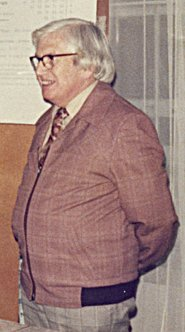
\includegraphics[height=\textheight]{pendlebury_only.jpg} &%
\fontsize{24pt}{24pt}\selectfont \textit{[Five] is not a multiple of
		two or three, so [it] does not normally crop up in
		calculations unless deliberately or unwittingly put
		there by us.\ldots Every third number in counting is
		a multiple of three, yet this vast category skips
		every power of ten!  All over the world every day by
		rounding off to hundreds, thousands, etc[.] people are
		rejecting multiples of three for multiples of five.
		Simple divisions then give recurring decimals or a
		rash of fives, and simple ratios become
		33\sfrac{1}{3}\%[,] 12\sfrac{1}{2}\%, etc.
		Unnecessarily awkward expressions all caused by
		counting in tens.}\par\vskip.5em \fontsize{18pt}{18pt}\selectfont \hbox{\textsc{\vbox{\hangafter=0\hangindent=2em%
	Tom Pendlebury}}}\\%
\end{tabular}%
\end{landscape}%
		\begin{landscape}
		\renewcommand*{\arraystretch}{1.2}
		\vspace{-1em}\centering\monthsty{July 11\e9}\vskip1em
		\noindent
		\begin{tabular}{|%
			>{\daysty\vspace{-.5em}}p{\daywidth}<{\vspace{-.8em}}|%
			>{\daysty\vspace{-.5em}}p{\daywidth}<{\vspace{-.8em}}|%
			>{\daysty\vspace{-.5em}}p{\daywidth}<{\vspace{-.8em}}|%
			>{\daysty\vspace{-.5em}}p{\daywidth}<{\vspace{-.8em}}|%
			>{\daysty\vspace{-.5em}}p{\daywidth}<{\vspace{-.8em}}|%
			>{\daysty\vspace{-.5em}}p{\daywidth}<{\vspace{-.8em}}|%
			>{\daysty\vspace{-.5em}}p{\daywidth}<{\vspace{-.8em}}|}
		\hline
		Sunday & Monday & Tuesday & Wednesday & Thursday%
		& Friday & Saturday \\
		\end{tabular}\vskip-1.4pt

\renewcommand*{\arraystretch}{1.2}
\noindent
\begin{tabular}{|p{\daywidth}|p{\daywidth}|%
p{\daywidth}|p{\daywidth}|p{\daywidth}|p{\daywidth}|%
p{\daywidth}|}
\hline
\multicolumn{1}{|c|}{
\hbox to 1\daywidth{%

	\hfil\hbox to\daywidth{%

		\vbox to.2\dayheight{\vskip2pt%

			\hbox to\daywidth{\hfil\thumbtitsty%

				June\hfil}\vskip2pt%

			\hbox to\daywidth{\hfil%

				\usebox{\monthsix}\hfil}%

		}%

	}\hfil%

}%

} &
\vtop to\dayheight {\hbox to \linewidth{\hfil\numsty 1\ls}
\rule{0pt}{\dayheight}}&\vtop to\dayheight {\hbox to \linewidth{\hfil\numsty 2\ls}
\rule{0pt}{\dayheight}}&\vtop to\dayheight {\hbox to \linewidth{\hfil\numsty 3\ls}
\rule{0pt}{\dayheight}}&\vtop to\dayheight {\hbox to \linewidth{\hfil\numsty 4\ls}
\rule{0pt}{\dayheight}}&\vtop to\dayheight {\hbox to \linewidth{\hfil\numsty 5\ls}
\rule{0pt}{\dayheight}}&\vtop to\dayheight {\hbox to \linewidth{\hfil\numsty 6\ls}
\rule{0pt}{\dayheight}}\\\hline
\vtop to\dayheight {\hbox to \linewidth{\hfil\numsty 7\ls}
\rule{0pt}{\dayheight}}&\vtop to\dayheight {\hbox to \linewidth{\hfil\numsty 8\ls}
\rule{0pt}{\dayheight}}&\vtop to\dayheight {\hbox to \linewidth{\hfil\numsty 9\ls}
\rule{0pt}{\dayheight}}&\vtop to\dayheight {\hbox to \linewidth{\hfil\numsty \x\ls}
\rule{0pt}{\dayheight}}&\vtop to\dayheight {\hbox to \linewidth{\hfil\numsty \e\ls}
\rule{0pt}{\dayheight}}&\vtop to\dayheight {\hbox to \linewidth{\hfil\numsty 10\ls}
\rule{0pt}{\dayheight}}&\vtop to\dayheight {\hbox to \linewidth{\hfil\numsty 11\ls}
\rule{0pt}{\dayheight}}\\\hline
\vtop to\dayheight {\hbox to \linewidth{\hfil\numsty 12\ls}
\rule{0pt}{\dayheight}}&\vtop to\dayheight {\hbox to \linewidth{\hfil\numsty 13\ls}
\rule{0pt}{\dayheight}}&\vtop to\dayheight {\hbox to \linewidth{\hfil\numsty 14\ls}
\rule{0pt}{\dayheight}}&\vtop to\dayheight {\hbox to \linewidth{\hfil\numsty 15\ls}
\rule{0pt}{\dayheight}}&\vtop to\dayheight {\hbox to \linewidth{\hfil\numsty 16\ls}
\rule{0pt}{\dayheight}}&\vtop to\dayheight {\hbox to \linewidth{\hfil\numsty 17\ls}
\rule{0pt}{\dayheight}}&\vtop to\dayheight {\hbox to \linewidth{\hfil\numsty 18\ls}
\rule{0pt}{\dayheight}}\\\hline
\vtop to\dayheight {\hbox to \linewidth{\hfil\numsty 19\ls}
\rule{0pt}{\dayheight}}&\vtop to\dayheight {\hbox to \linewidth{\hfil\numsty 1\x\ls}
\rule{0pt}{\dayheight}}&\vtop to\dayheight {\hbox to \linewidth{\hfil\numsty 1\e\ls}
\rule{0pt}{\dayheight}}&\vtop to\dayheight {\hbox to \linewidth{\hfil\numsty 20\ls}
\rule{0pt}{\dayheight}}&\vtop to\dayheight {\hbox to \linewidth{\hfil\numsty 21\ls}
\rule{0pt}{\dayheight}}&\vtop to\dayheight {\hbox to \linewidth{\hfil\numsty 22\ls}
\rule{0pt}{\dayheight}}&\vtop to\dayheight {\hbox to \linewidth{\hfil\numsty 23\ls}
\rule{0pt}{\dayheight}}\\\hline
\vtop to\dayheight {\hbox to \linewidth{\hfil\numsty 24\ls}
\rule{0pt}{\dayheight}}&\vtop to\dayheight {\hbox to \linewidth{\hfil\numsty 25\ls}
\rule{0pt}{\dayheight}}&\vtop to\dayheight {\hbox to \linewidth{\hfil\numsty 26\ls}
\rule{0pt}{\dayheight}}&\vtop to\dayheight {\hbox to \linewidth{\hfil\numsty 27\ls}
\rule{0pt}{\dayheight}}&\multicolumn{3}{c|}{
\hbox to 3\daywidth{%

	\hfil\hbox to\daywidth{%

		\vbox to.2\dayheight{\vskip2pt%

			\hbox to\daywidth{\hfil\thumbtitsty%

				June\hfil}\vskip2pt%

			\hbox to\daywidth{\hfil%

				\usebox{\monthsix}\hfil}%

		}%

	}%

	\hfil\hbox to\daywidth{%

		\vbox to.2\dayheight{\vskip2pt%

			\hbox to\daywidth{\hfil\thumbtitsty%

				August\hfil}\vskip2pt%

			\hbox to\daywidth{\hfil%

				\usebox{\montheight}\hfil}%

		}%

	}\hfil%

}%

} &
\hline\end{tabular}
\end{landscape}
\newpage
\begin{landscape}%
\renewcommand{\tabcolsep}{1em}%
\begin{tabular*}{\textwidth}{>{\hfil}m{.47\linewidth}<{\hfil}m{.47\linewidth}}%
\includegraphics[height=\textheight]{weights_dozenal.mps} &%
\fontsize{24pt}{24pt}\selectfont \textit{Just as with pure
		binary, all intermediate weights can be achieved by
		combining others, so we need only one of each size.
		[But] [t]here is more.  It will not have gone
		unobserved that [0;]3[], [0;]6[] and 1[] can be made
		from combinations of lower values; in fact, if we
		needed to go only as far as a dozen[], the 1[] weight
		would be superfluous.  Including the 1[], therefore,
		allows further weighing up to and including 2\ldots
		\emph{without the need for a 2[] piece}.  If the 2[]
		is included, the range extends to 4[]
		\emph{inclusive}.\ldots while the binary misses by
		\sfrac{1}{2}.\ldots The decimal set\ldots involves
		nine weights rather than seven\ldots}\par\vskip.5em \fontsize{18pt}{18pt}\selectfont \hbox{\textsc{\vbox{\hangafter=0\hangindent=2em%
	Troy, DSGB}}}\\%
\end{tabular}%
\end{landscape}%
		\begin{landscape}
		\renewcommand*{\arraystretch}{1.2}
		\vspace{-1em}\centering\monthsty{August 11\e9}\vskip1em
		\noindent
		\begin{tabular}{|%
			>{\daysty\vspace{-.5em}}p{\daywidth}<{\vspace{-.8em}}|%
			>{\daysty\vspace{-.5em}}p{\daywidth}<{\vspace{-.8em}}|%
			>{\daysty\vspace{-.5em}}p{\daywidth}<{\vspace{-.8em}}|%
			>{\daysty\vspace{-.5em}}p{\daywidth}<{\vspace{-.8em}}|%
			>{\daysty\vspace{-.5em}}p{\daywidth}<{\vspace{-.8em}}|%
			>{\daysty\vspace{-.5em}}p{\daywidth}<{\vspace{-.8em}}|%
			>{\daysty\vspace{-.5em}}p{\daywidth}<{\vspace{-.8em}}|}
		\hline
		Sunday & Monday & Tuesday & Wednesday & Thursday%
		& Friday & Saturday \\
		\end{tabular}\vskip-1.4pt

\renewcommand*{\arraystretch}{1.2}
\noindent
\begin{tabular}{|p{\daywidth}|p{\daywidth}|%
p{\daywidth}|p{\daywidth}|p{\daywidth}|p{\daywidth}|%
p{\daywidth}|}
\hline
\multicolumn{4}{|c|}{
\hbox to 4\daywidth{%

	\hfil\hbox to\daywidth{%

		\vbox to.2\dayheight{\vskip2pt%

			\hbox to\daywidth{\hfil\thumbtitsty%

				July\hfil}\vskip2pt%

			\hbox to\daywidth{\hfil%

				\usebox{\monthseven}\hfil}%

		}%

	}%

	\hfil\hbox to\daywidth{%

		\vbox to.2\dayheight{\vskip2pt%

			\hbox to\daywidth{\hfil\thumbtitsty%

				September\hfil}\vskip2pt%

			\hbox to\daywidth{\hfil%

				\usebox{\monthnine}\hfil}%

		}%

	}\hfil%

}%

} &
\vtop to\dayheight {\hbox to \linewidth{\hfil\numsty 1\ls}
\rule{0pt}{\dayheight}}&\vtop to\dayheight {\hbox to \linewidth{\hfil\numsty 2\ls}
\rule{0pt}{\dayheight}}&\vtop to\dayheight {\hbox to \linewidth{\hfil\numsty 3\ls}
\rule{0pt}{\dayheight}}\\\hline
\vtop to\dayheight {\hbox to \linewidth{\hfil\numsty 4\ls}
\rule{0pt}{\dayheight}}&\vtop to\dayheight {\hbox to \linewidth{\hfil\numsty 5\ls}
\rule{0pt}{\dayheight}}&\vtop to\dayheight {\hbox to \linewidth{\hfil\numsty 6\ls}
\rule{0pt}{\dayheight}}&\vtop to\dayheight {\hbox to \linewidth{\hfil\numsty 7\ls}
\rule{0pt}{\dayheight}}&\vtop to\dayheight {\hbox to \linewidth{\hfil\numsty 8\ls}
\rule{0pt}{\dayheight}}&\vtop to\dayheight {\hbox to \linewidth{\hfil\numsty 9\ls}
\rule{0pt}{\dayheight}}&\vtop to\dayheight {\hbox to \linewidth{\hfil\numsty \x\ls}
\rule{0pt}{\dayheight}}\\\hline
\vtop to\dayheight {\hbox to \linewidth{\hfil\numsty \e\ls}
\rule{0pt}{\dayheight}}&\vtop to\dayheight {\hbox to \linewidth{\hfil\numsty 10\ls}
\rule{0pt}{\dayheight}}&\vtop to\dayheight {\hbox to \linewidth{\hfil\numsty 11\ls}
\rule{0pt}{\dayheight}}&\vtop to\dayheight {\hbox to \linewidth{\hfil\numsty 12\ls}
\rule{0pt}{\dayheight}}&\vtop to\dayheight {\hbox to \linewidth{\hfil\numsty 13\ls}
\rule{0pt}{\dayheight}}&\vtop to\dayheight {\hbox to \linewidth{\hfil\numsty 14\ls}
\rule{0pt}{\dayheight}}&\vtop to\dayheight {\hbox to \linewidth{\hfil\numsty 15\ls}
\rule{0pt}{\dayheight}}\\\hline
\vtop to\dayheight {\hbox to \linewidth{\hfil\numsty 16\ls}
\rule{0pt}{\dayheight}}&\vtop to\dayheight {\hbox to \linewidth{\hfil\numsty 17\ls}
\rule{0pt}{\dayheight}}&\vtop to\dayheight {\hbox to \linewidth{\hfil\numsty 18\ls}
\rule{0pt}{\dayheight}}&\vtop to\dayheight {\hbox to \linewidth{\hfil\numsty 19\ls}
\rule{0pt}{\dayheight}}&\vtop to\dayheight {\hbox to \linewidth{\hfil\numsty 1\x\ls}
\rule{0pt}{\dayheight}}&\vtop to\dayheight {\hbox to \linewidth{\hfil\numsty 1\e\ls}
\rule{0pt}{\dayheight}}&\vtop to\dayheight {\hbox to \linewidth{\hfil\numsty 20\ls}
\rule{0pt}{\dayheight}}\\\hline
\vtop to\dayheight {\hbox to \linewidth{\hfil\numsty 21\ls}
\rule{0pt}{\dayheight}}&\vtop to\dayheight {\hbox to \linewidth{\hfil\numsty 22\ls}
\rule{0pt}{\dayheight}}&\vtop to\dayheight {\hbox to \linewidth{\hfil\numsty 23\ls}
\rule{0pt}{\dayheight}}&\vtop to\dayheight {\hbox to \linewidth{\hfil\numsty 24\ls}
\rule{0pt}{\dayheight}}&\vtop to\dayheight {\hbox to \linewidth{\hfil\numsty 25\ls}
\rule{0pt}{\dayheight}}&\vtop to\dayheight {\hbox to \linewidth{\hfil\numsty 26\ls}
\rule{0pt}{\dayheight}}&\vtop to\dayheight {\hbox to \linewidth{\hfil\numsty 27\ls}
\rule{0pt}{\dayheight}}\\\hline\end{tabular}
\end{landscape}
\newpage
\begin{landscape}%
\renewcommand{\tabcolsep}{1em}%
\vspace*{\stretch{1}}%
\begin{tabular*}{\textwidth}{>{\hfil}m{.47\linewidth}<{\hfil}m{.47\linewidth}}%
\includegraphics[height=0.65\textheight]{prime_circle.mps} &%
\fontsize{24pt}{24pt}\selectfont \textit{Hence, the set of
		natural numbers terminating with 1, 5, 7 or \e\ must
		contain all prime numbers greater than 3, and excludes
		all odd numbers divisible by 3.   It follows that this
		is the \emph{minimum} set to contain \emph{all}
		primes greater than 3.  Rearranging the terminal
		digits as 5, 7 and \e, 1 shows the set to be of the
		form:  $(6n\pm1)$\ldots The fact [is] that
		prime-number positions are \emph{completely}
		controlled by 6 (itself the product of 2 and 3, and
		the companion of our dozenal base).}\par\vskip.5em \fontsize{18pt}{18pt}\selectfont \hbox{\textsc{\vbox{\hangafter=0\hangindent=2em%
	Don
		Hammond}}}\\%
\end{tabular}%
\vspace*{\stretch{1}}%
\end{landscape}%
		\begin{landscape}
		\renewcommand*{\arraystretch}{1.2}
		\vspace{-1em}\centering\monthsty{September 11\e9}\vskip1em
		\noindent
		\begin{tabular}{|%
			>{\daysty\vspace{-.5em}}p{\daywidth}<{\vspace{-.8em}}|%
			>{\daysty\vspace{-.5em}}p{\daywidth}<{\vspace{-.8em}}|%
			>{\daysty\vspace{-.5em}}p{\daywidth}<{\vspace{-.8em}}|%
			>{\daysty\vspace{-.5em}}p{\daywidth}<{\vspace{-.8em}}|%
			>{\daysty\vspace{-.5em}}p{\daywidth}<{\vspace{-.8em}}|%
			>{\daysty\vspace{-.5em}}p{\daywidth}<{\vspace{-.8em}}|%
			>{\daysty\vspace{-.5em}}p{\daywidth}<{\vspace{-.8em}}|}
		\hline
		Sunday & Monday & Tuesday & Wednesday & Thursday%
		& Friday & Saturday \\
		\end{tabular}\vskip-1.4pt

\renewcommand*{\arraystretch}{1.2}
\noindent
\begin{tabular}{|p{\daywidth}|p{\daywidth}|%
p{\daywidth}|p{\daywidth}|p{\daywidth}|p{\daywidth}|%
p{\daywidth}|}
\hline
\vtop to\dayheight {\hbox to \linewidth{\hfil\numsty 1\ls}
\rule{0pt}{\dayheight}}&\vtop to\dayheight {\hbox to \linewidth{\hfil\numsty 2\ls}
\rule{0pt}{\dayheight}}&\vtop to\dayheight {\hbox to \linewidth{\hfil\numsty 3\ls}
\rule{0pt}{\dayheight}}&\vtop to\dayheight {\hbox to \linewidth{\hfil\numsty 4\ls}
\rule{0pt}{\dayheight}}&\vtop to\dayheight {\hbox to \linewidth{\hfil\numsty 5\ls}
\rule{0pt}{\dayheight}}&\vtop to\dayheight {\hbox to \linewidth{\hfil\numsty 6\ls}
\rule{0pt}{\dayheight}}&\vtop to\dayheight {\hbox to \linewidth{\hfil\numsty 7\ls}
\rule{0pt}{\dayheight}}\\\hline
\vtop to\dayheight {\hbox to \linewidth{\hfil\numsty 8\ls}
\rule{0pt}{\dayheight}}&\vtop to\dayheight {\hbox to \linewidth{\hfil\numsty 9\ls}
\rule{0pt}{\dayheight}}&\vtop to\dayheight {\hbox to \linewidth{\hfil\numsty \x\ls}
\rule{0pt}{\dayheight}}&\vtop to\dayheight {\hbox to \linewidth{\hfil\numsty \e\ls}
\rule{0pt}{\dayheight}}&\vtop to\dayheight {\hbox to \linewidth{\hfil\numsty 10\ls}
\rule{0pt}{\dayheight}}&\vtop to\dayheight {\hbox to \linewidth{\hfil\numsty 11\ls}
\rule{0pt}{\dayheight}}&\vtop to\dayheight {\hbox to \linewidth{\hfil\numsty 12\ls}
\rule{0pt}{\dayheight}}\\\hline
\vtop to\dayheight {\hbox to \linewidth{\hfil\numsty 13\ls}
\rule{0pt}{\dayheight}}&\vtop to\dayheight {\hbox to \linewidth{\hfil\numsty 14\ls}
\rule{0pt}{\dayheight}}&\vtop to\dayheight {\hbox to \linewidth{\hfil\numsty 15\ls}
\rule{0pt}{\dayheight}}&\vtop to\dayheight {\hbox to \linewidth{\hfil\numsty 16\ls}
\rule{0pt}{\dayheight}}&\vtop to\dayheight {\hbox to \linewidth{\hfil\numsty 17\ls}
\rule{0pt}{\dayheight}}&\vtop to\dayheight {\hbox to \linewidth{\hfil\numsty 18\ls}
\rule{0pt}{\dayheight}}&\vtop to\dayheight {\hbox to \linewidth{\hfil\numsty 19\ls}
\rule{0pt}{\dayheight}}\\\hline
\vtop to\dayheight {\hbox to \linewidth{\hfil\numsty 1\x\ls}
\rule{0pt}{\dayheight}}&\vtop to\dayheight {\hbox to \linewidth{\hfil\numsty 1\e\ls}
\rule{0pt}{\dayheight}}&\vtop to\dayheight {\hbox to \linewidth{\hfil\numsty 20\ls}
\rule{0pt}{\dayheight}}&\vtop to\dayheight {\hbox to \linewidth{\hfil\numsty 21\ls}
\rule{0pt}{\dayheight}}&\vtop to\dayheight {\hbox to \linewidth{\hfil\numsty 22\ls}
\rule{0pt}{\dayheight}}&\vtop to\dayheight {\hbox to \linewidth{\hfil\numsty 23\ls}
\rule{0pt}{\dayheight}}&\vtop to\dayheight {\hbox to \linewidth{\hfil\numsty 24\ls}
\rule{0pt}{\dayheight}}\\\hline
\vtop to\dayheight {\hbox to \linewidth{\hfil\numsty 25\ls}
\rule{0pt}{\dayheight}}&\vtop to\dayheight {\hbox to \linewidth{\hfil\numsty 26\ls}
\rule{0pt}{\dayheight}}&\multicolumn{5}{c|}{
\hbox to 5\daywidth{%

	\hfil\hbox to\daywidth{%

		\vbox to.2\dayheight{\vskip2pt%

			\hbox to\daywidth{\hfil\thumbtitsty%

				August\hfil}\vskip2pt%

			\hbox to\daywidth{\hfil%

				\usebox{\montheight}\hfil}%

		}%

	}%

	\hfil\hbox to\daywidth{%

		\vbox to.2\dayheight{\vskip2pt%

			\hbox to\daywidth{\hfil\thumbtitsty%

				October\hfil}\vskip2pt%

			\hbox to\daywidth{\hfil%

				\usebox{\monthten}\hfil}%

		}%

	}\hfil%

}%

} &
\hline\end{tabular}
\end{landscape}
\newpage
\begin{landscape}%
\renewcommand{\tabcolsep}{1em}%
\begin{tabular*}{\textwidth}{>{\hfil}m{.47\linewidth}<{\hfil}m{.47\linewidth}}%
\includegraphics[height=\textheight]{newcansort.mps} &%
\fontsize{24pt}{24pt}\selectfont \textit{Packing in dozens shows an
		immediate advantage\ldots [t]he cost per can (or
		other object) of cardboard increases by more than
		\x\ per gross (over 7 per cent in decimal terms) by
		changing from dozens to decimal packing.\ldots The
		really decisive example is the two-layer form (allowed
		by the factorability of the dozen) in which the
		\emph{total} enclosure area is less than the
		requirement for ten.\ldots [S]uch cans are so much
		more cheaply packed by the dozen than in tens that a
		twelve-pack with two empty spaces actually costs less
		than a ten-pack completely filled!}\par\vskip.5em \fontsize{18pt}{18pt}\selectfont \hbox{\textsc{\vbox{\hangafter=0\hangindent=2em%
	Troy,
		DSGB}}}\\%
\end{tabular}%
\end{landscape}%
		\begin{landscape}
		\renewcommand*{\arraystretch}{1.2}
		\vspace{-1em}\centering\monthsty{October 11\e9}\vskip1em
		\noindent
		\begin{tabular}{|%
			>{\daysty\vspace{-.5em}}p{\daywidth}<{\vspace{-.8em}}|%
			>{\daysty\vspace{-.5em}}p{\daywidth}<{\vspace{-.8em}}|%
			>{\daysty\vspace{-.5em}}p{\daywidth}<{\vspace{-.8em}}|%
			>{\daysty\vspace{-.5em}}p{\daywidth}<{\vspace{-.8em}}|%
			>{\daysty\vspace{-.5em}}p{\daywidth}<{\vspace{-.8em}}|%
			>{\daysty\vspace{-.5em}}p{\daywidth}<{\vspace{-.8em}}|%
			>{\daysty\vspace{-.5em}}p{\daywidth}<{\vspace{-.8em}}|}
		\hline
		Sunday & Monday & Tuesday & Wednesday & Thursday%
		& Friday & Saturday \\
		\end{tabular}\vskip-1.4pt

\renewcommand*{\arraystretch}{1.2}
\noindent
\begin{tabular}{|p{\daywidth}|p{\daywidth}|%
p{\daywidth}|p{\daywidth}|p{\daywidth}|p{\daywidth}|%
p{\daywidth}|}
\hline
\multicolumn{2}{|c|}{
\hbox to 2\daywidth{%

	\hfil\hbox to\daywidth{%

		\vbox to.2\dayheight{\vskip2pt%

			\hbox to\daywidth{\hfil\thumbtitsty%

				September\hfil}\vskip2pt%

			\hbox to\daywidth{\hfil%

				\usebox{\monthnine}\hfil}%

		}%

	}\hfil%

}%

} &
\vtop to\dayheight {\hbox to \linewidth{\hfil\numsty 1\ls}
\rule{0pt}{\dayheight}}&\vtop to\dayheight {\hbox to \linewidth{\hfil\numsty 2\ls}
\rule{0pt}{\dayheight}}&\vtop to\dayheight {\hbox to \linewidth{\hfil\numsty 3\ls}
\rule{0pt}{\dayheight}}&\vtop to\dayheight {\hbox to \linewidth{\hfil\numsty 4\ls}
\rule{0pt}{\dayheight}}&\vtop to\dayheight {\hbox to \linewidth{\hfil\numsty 5\ls}
\rule{0pt}{\dayheight}}\\\hline
\vtop to\dayheight {\hbox to \linewidth{\hfil\numsty 6\ls}
\rule{0pt}{\dayheight}}&\vtop to\dayheight {\hbox to \linewidth{\hfil\numsty 7\ls}
\rule{0pt}{\dayheight}}&\vtop to\dayheight {\hbox to \linewidth{\hfil\numsty 8\ls}
\rule{0pt}{\dayheight}}&\vtop to\dayheight {\hbox to \linewidth{\hfil\numsty 9\ls}
\rule{0pt}{\dayheight}}&\vtop to\dayheight {\hbox to \linewidth{\hfil\numsty \x\ls}
\rule{0pt}{\dayheight}}&\vtop to\dayheight {\hbox to \linewidth{\hfil\numsty \e\ls}
\rule{0pt}{\dayheight}}&\vtop to\dayheight {\hbox to \linewidth{\hfil\numsty 10\ls}
\rule{0pt}{\dayheight}}\\\hline
\vtop to\dayheight {\hbox to \linewidth{\hfil\numsty 11\ls}
\rule{0pt}{\dayheight}}&\vtop to\dayheight {\hbox to \linewidth{\hfil\numsty 12\ls}
\rule{0pt}{\dayheight}}&\vtop to\dayheight {\hbox to \linewidth{\hfil\numsty 13\ls}
\rule{0pt}{\dayheight}}&\vtop to\dayheight {\hbox to \linewidth{\hfil\numsty 14\ls}
\rule{0pt}{\dayheight}}&\vtop to\dayheight {\hbox to \linewidth{\hfil\numsty 15\ls}
\rule{0pt}{\dayheight}}&\vtop to\dayheight {\hbox to \linewidth{\hfil\numsty 16\ls}
\rule{0pt}{\dayheight}}&\vtop to\dayheight {\hbox to \linewidth{\hfil\numsty 17\ls}
\rule{0pt}{\dayheight}}\\\hline
\vtop to\dayheight {\hbox to \linewidth{\hfil\numsty 18\ls}
\rule{0pt}{\dayheight}}&\vtop to\dayheight {\hbox to \linewidth{\hfil\numsty 19\ls}
\rule{0pt}{\dayheight}}&\vtop to\dayheight {\hbox to \linewidth{\hfil\numsty 1\x\ls}
\rule{0pt}{\dayheight}}&\vtop to\dayheight {\hbox to \linewidth{\hfil\numsty 1\e\ls}
\rule{0pt}{\dayheight}}&\vtop to\dayheight {\hbox to \linewidth{\hfil\numsty 20\ls}
\rule{0pt}{\dayheight}}&\vtop to\dayheight {\hbox to \linewidth{\hfil\numsty 21\ls}
\rule{0pt}{\dayheight}}&\vtop to\dayheight {\hbox to \linewidth{\hfil\numsty 22\ls}
\rule{0pt}{\dayheight}}\\\hline
\vtop to\dayheight {\hbox to \linewidth{\hfil\numsty 23\ls}
\rule{0pt}{\dayheight}}&\vtop to\dayheight {\hbox to \linewidth{\hfil\numsty 24\ls}
\rule{0pt}{\dayheight}}&\vtop to\dayheight {\hbox to \linewidth{\hfil\numsty 25\ls}
\rule{0pt}{\dayheight}}&\vtop to\dayheight {\hbox to \linewidth{\hfil\numsty 26\ls}
\rule{0pt}{\dayheight}}&\vtop to\dayheight {\hbox to \linewidth{\hfil\numsty 27\ls}
\rule{0pt}{\dayheight}}&\multicolumn{2}{c|}{
\hbox to 2\daywidth{%

	\hfil\hbox to\daywidth{%

		\vbox to.2\dayheight{\vskip2pt%

			\hbox to\daywidth{\hfil\thumbtitsty%

				November\hfil}\vskip2pt%

			\hbox to\daywidth{\hfil%

				\usebox{\monthelv}\hfil}%

		}%

	}\hfil%

}%

} &
\hline\end{tabular}
\end{landscape}
\newpage
\begin{landscape}%
\renewcommand{\tabcolsep}{1em}%
\vspace*{\stretch{1}}%
\begin{tabular*}{\textwidth}{>{\hfil}m{.47\linewidth}<{\hfil}m{.47\linewidth}}%

\includegraphics[height=0.8\textheight]{newpalm1.png} &%
\fontsize{24pt}{24pt}\selectfont \textit{[We can] count[] on the
		segments (phalanges) of the fingers.  If one uses the
		thumb as a pointer, one can easily count to twelve on
		one hand.}\par\vskip.5em \fontsize{18pt}{18pt}\selectfont \hbox{\textsc{\vbox{\hangafter=0\hangindent=2em%
	Prof.\ Gene Zirkel}}}\\%
\end{tabular}%
\vspace*{\stretch{1}}%
\end{landscape}%
		\begin{landscape}
		\renewcommand*{\arraystretch}{1.2}
		\vspace{-1em}\centering\monthsty{November 11\e9}\vskip1em
		\noindent
		\begin{tabular}{|%
			>{\daysty\vspace{-.5em}}p{\daywidth}<{\vspace{-.8em}}|%
			>{\daysty\vspace{-.5em}}p{\daywidth}<{\vspace{-.8em}}|%
			>{\daysty\vspace{-.5em}}p{\daywidth}<{\vspace{-.8em}}|%
			>{\daysty\vspace{-.5em}}p{\daywidth}<{\vspace{-.8em}}|%
			>{\daysty\vspace{-.5em}}p{\daywidth}<{\vspace{-.8em}}|%
			>{\daysty\vspace{-.5em}}p{\daywidth}<{\vspace{-.8em}}|%
			>{\daysty\vspace{-.5em}}p{\daywidth}<{\vspace{-.8em}}|}
		\hline
		Sunday & Monday & Tuesday & Wednesday & Thursday%
		& Friday & Saturday \\
		\end{tabular}\vskip-1.4pt

\renewcommand*{\arraystretch}{1.2}
\noindent
\begin{tabular}{|p{\daywidth}|p{\daywidth}|%
p{\daywidth}|p{\daywidth}|p{\daywidth}|p{\daywidth}|%
p{\daywidth}|}
\hline
\multicolumn{5}{|c|}{
\hbox to 5\daywidth{%

	\hfil\hbox to\daywidth{%

		\vbox to.2\dayheight{\vskip2pt%

			\hbox to\daywidth{\hfil\thumbtitsty%

				October\hfil}\vskip2pt%

			\hbox to\daywidth{\hfil%

				\usebox{\monthten}\hfil}%

		}%

	}%

	\hfil\hbox to\daywidth{%

		\vbox to.2\dayheight{\vskip2pt%

			\hbox to\daywidth{\hfil\thumbtitsty%

				December\hfil}\vskip2pt%

			\hbox to\daywidth{\hfil%

				\usebox{\monthunqua}\hfil}%

		}%

	}\hfil%

}%

} &
\vtop to\dayheight {\hbox to \linewidth{\hfil\numsty 1\ls}
\rule{0pt}{\dayheight}}&\vtop to\dayheight {\hbox to \linewidth{\hfil\numsty 2\ls}
\rule{0pt}{\dayheight}}\\\hline
\vtop to\dayheight {\hbox to \linewidth{\hfil\numsty 3\ls}
\rule{0pt}{\dayheight}}&\vtop to\dayheight {\hbox to \linewidth{\hfil\numsty 4\ls}
\rule{0pt}{\dayheight}}&\vtop to\dayheight {\hbox to \linewidth{\hfil\numsty 5\ls}
\rule{0pt}{\dayheight}}&\vtop to\dayheight {\hbox to \linewidth{\hfil\numsty 6\ls}
\rule{0pt}{\dayheight}}&\vtop to\dayheight {\hbox to \linewidth{\hfil\numsty 7\ls}
\rule{0pt}{\dayheight}}&\vtop to\dayheight {\hbox to \linewidth{\hfil\numsty 8\ls}
\rule{0pt}{\dayheight}}&\vtop to\dayheight {\hbox to \linewidth{\hfil\numsty 9\ls}
\rule{0pt}{\dayheight}}\\\hline
\vtop to\dayheight {\hbox to \linewidth{\hfil\numsty \x\ls}
\rule{0pt}{\dayheight}}&\vtop to\dayheight {\hbox to \linewidth{\hfil\numsty \e\ls}
\rule{0pt}{\dayheight}}&\vtop to\dayheight {\hbox to \linewidth{\hfil\numsty 10\ls}
\rule{0pt}{\dayheight}}&\vtop to\dayheight {\hbox to \linewidth{\hfil\numsty 11\ls}
\rule{0pt}{\dayheight}}&\vtop to\dayheight {\hbox to \linewidth{\hfil\numsty 12\ls}
\rule{0pt}{\dayheight}}&\vtop to\dayheight {\hbox to \linewidth{\hfil\numsty 13\ls}
\rule{0pt}{\dayheight}}&\vtop to\dayheight {\hbox to \linewidth{\hfil\numsty 14\ls}
\rule{0pt}{\dayheight}}\\\hline
\vtop to\dayheight {\hbox to \linewidth{\hfil\numsty 15\ls}
\rule{0pt}{\dayheight}}&\vtop to\dayheight {\hbox to \linewidth{\hfil\numsty 16\ls}
\rule{0pt}{\dayheight}}&\vtop to\dayheight {\hbox to \linewidth{\hfil\numsty 17\ls}
\rule{0pt}{\dayheight}}&\vtop to\dayheight {\hbox to \linewidth{\hfil\numsty 18\ls}
\rule{0pt}{\dayheight}}&\vtop to\dayheight {\hbox to \linewidth{\hfil\numsty 19\ls}
\rule{0pt}{\dayheight}}&\vtop to\dayheight {\hbox to \linewidth{\hfil\numsty 1\x\ls}
\rule{0pt}{\dayheight}}&\vtop to\dayheight {\hbox to \linewidth{\hfil\numsty 1\e\ls}
\rule{0pt}{\dayheight}}\\\hline
\vtop to\dayheight {\hbox to \linewidth{\hfil\numsty 20\ls}
\rule{0pt}{\dayheight}}&\vtop to\dayheight {\hbox to \linewidth{\hfil\numsty 21\ls}
\rule{0pt}{\dayheight}}&\vtop to\dayheight {\hbox to \linewidth{\hfil\numsty 22\ls}
\rule{0pt}{\dayheight}}&\vtop to\dayheight {\hbox to \linewidth{\hfil\numsty 23\ls}
\rule{0pt}{\dayheight}}&\vtop to\dayheight {\hbox to \linewidth{\hfil\numsty 24\ls}
\rule{0pt}{\dayheight}}&\vtop to\dayheight {\hbox to \linewidth{\hfil\numsty 25\ls}
\rule{0pt}{\dayheight}}&\vtop to\dayheight {\hbox to \linewidth{\hfil\numsty 26\ls}
\rule{0pt}{\dayheight}}\\\hline\end{tabular}
\end{landscape}
\newpage
\begin{landscape}%
\renewcommand{\tabcolsep}{1em}%
\vspace*{\stretch{1}}%
\begin{tabular*}{\textwidth}{>{\hfil}m{.47\linewidth}<{\hfil}m{.47\linewidth}}%
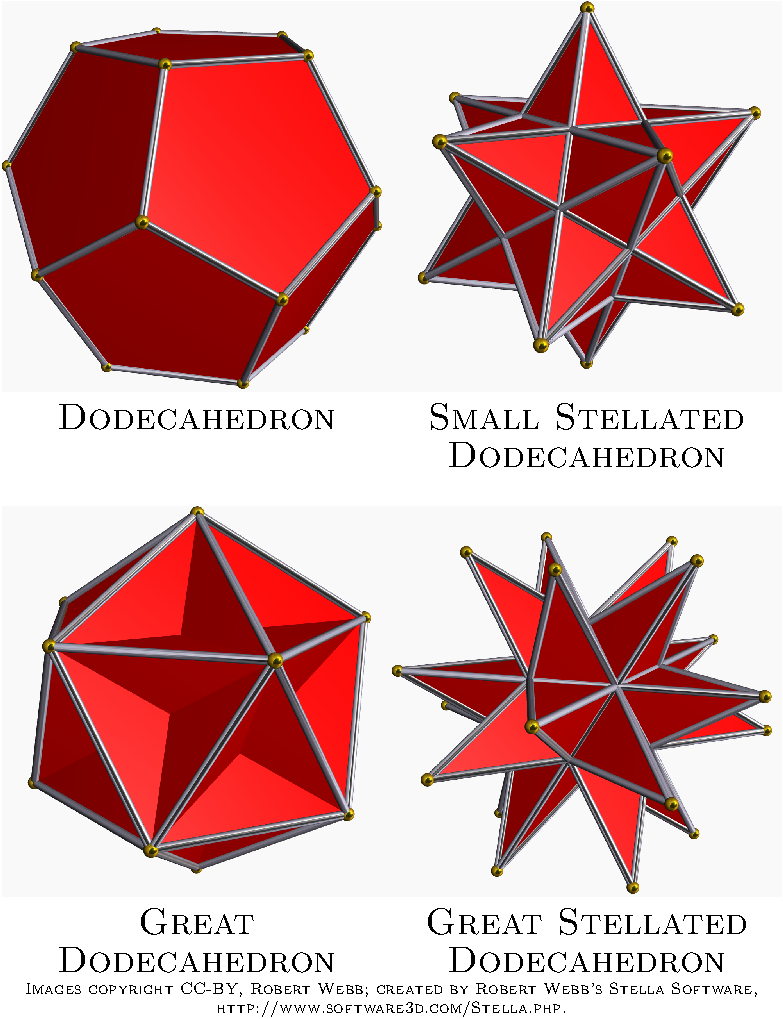
\includegraphics[height=0.85\textheight]{regular_polyhedra-crop.pdf} &%
\fontsize{24pt}{24pt}\selectfont \textit{Of the nine regular
		polyhedra, fully four of them are built upon the
		number twelve:  the dodecahedron, the small stellated
		dodecahedron, the great dodecahedron, and the great
		stellated dodecahedron.  Two more, the tetrahedron and
		the cube, are built upon the factors of twelve.  Five
		only becomes important when it is paired with twelve
		in the dodecahedron; ten is \emph{never} important.
		We must get to the icosahedron, at twenty, before ten
		plays into the question at all.}\par\vskip.5em \fontsize{18pt}{18pt}\selectfont \hbox{\textsc{\vbox{\hangafter=0\hangindent=2em%
	}}}\\%
\end{tabular}%
\vspace*{\stretch{1}}%
\end{landscape}%
		\begin{landscape}
		\renewcommand*{\arraystretch}{1.2}
		\vspace{-1em}\centering\monthsty{December 11\e9}\vskip1em
		\noindent
		\begin{tabular}{|%
			>{\daysty\vspace{-.5em}}p{\daywidth}<{\vspace{-.8em}}|%
			>{\daysty\vspace{-.5em}}p{\daywidth}<{\vspace{-.8em}}|%
			>{\daysty\vspace{-.5em}}p{\daywidth}<{\vspace{-.8em}}|%
			>{\daysty\vspace{-.5em}}p{\daywidth}<{\vspace{-.8em}}|%
			>{\daysty\vspace{-.5em}}p{\daywidth}<{\vspace{-.8em}}|%
			>{\daysty\vspace{-.5em}}p{\daywidth}<{\vspace{-.8em}}|%
			>{\daysty\vspace{-.5em}}p{\daywidth}<{\vspace{-.8em}}|}
		\hline
		Sunday & Monday & Tuesday & Wednesday & Thursday%
		& Friday & Saturday \\
		\end{tabular}\vskip-1.4pt

\renewcommand*{\arraystretch}{1.2}
\noindent
\begin{tabular}{|p{\daywidth}|p{\daywidth}|%
p{\daywidth}|p{\daywidth}|p{\daywidth}|p{\daywidth}|%
p{\daywidth}|}
\hline
\vtop to\dayheight {\hbox to \linewidth{\hfil\numsty 1\ls}
\rule{0pt}{\dayheight}}&\vtop to\dayheight {\hbox to \linewidth{\hfil\numsty 2\ls}
\rule{0pt}{\dayheight}}&\vtop to\dayheight {\hbox to \linewidth{\hfil\numsty 3\ls}
\rule{0pt}{\dayheight}}&\vtop to\dayheight {\hbox to \linewidth{\hfil\numsty 4\ls}
\rule{0pt}{\dayheight}}&\vtop to\dayheight {\hbox to \linewidth{\hfil\numsty 5\ls}
\rule{0pt}{\dayheight}}&\vtop to\dayheight {\hbox to \linewidth{\hfil\numsty 6\ls}
\rule{0pt}{\dayheight}}&\vtop to\dayheight {\hbox to \linewidth{\hfil\numsty 7\ls}
\rule{0pt}{\dayheight}}\\\hline
\vtop to\dayheight {\hbox to \linewidth{\hfil\numsty 8\ls}
\rule{0pt}{\dayheight}}&\vtop to\dayheight {\hbox to \linewidth{\hfil\numsty 9\ls}
\rule{0pt}{\dayheight}}&\vtop to\dayheight {\hbox to \linewidth{\hfil\numsty \x\ls}
\rule{0pt}{\dayheight}}&\vtop to\dayheight {\hbox to \linewidth{\hfil\numsty \e\ls}
\rule{0pt}{\dayheight}}&\vtop to\dayheight {\hbox to \linewidth{\hfil\numsty 10\ls}
\rule{0pt}{\dayheight}}&\vtop to\dayheight {\hbox to \linewidth{\hfil\numsty 11\ls}
\rule{0pt}{\dayheight}}&\vtop to\dayheight {\hbox to \linewidth{\hfil\numsty 12\ls}
\rule{0pt}{\dayheight}}\\\hline
\vtop to\dayheight {\hbox to \linewidth{\hfil\numsty 13\ls}
\rule{0pt}{\dayheight}}&\vtop to\dayheight {\hbox to \linewidth{\hfil\numsty 14\ls}
\rule{0pt}{\dayheight}}&\vtop to\dayheight {\hbox to \linewidth{\hfil\numsty 15\ls}
\rule{0pt}{\dayheight}}&\vtop to\dayheight {\hbox to \linewidth{\hfil\numsty 16\ls}
\rule{0pt}{\dayheight}}&\vtop to\dayheight {\hbox to \linewidth{\hfil\numsty 17\ls}
\rule{0pt}{\dayheight}}&\vtop to\dayheight {\hbox to \linewidth{\hfil\numsty 18\ls}
\rule{0pt}{\dayheight}}&\vtop to\dayheight {\hbox to \linewidth{\hfil\numsty 19\ls}
\rule{0pt}{\dayheight}}\\\hline
\vtop to\dayheight {\hbox to \linewidth{\hfil\numsty 1\x\ls}
\rule{0pt}{\dayheight}}&\vtop to\dayheight {\hbox to \linewidth{\hfil\numsty 1\e\ls}
\rule{0pt}{\dayheight}}&\vtop to\dayheight {\hbox to \linewidth{\hfil\numsty 20\ls}
\rule{0pt}{\dayheight}}&\vtop to\dayheight {\hbox to \linewidth{\hfil\numsty 21\ls}
\rule{0pt}{\dayheight}}&\vtop to\dayheight {\hbox to \linewidth{\hfil\numsty 22\ls}
\rule{0pt}{\dayheight}}&\vtop to\dayheight {\hbox to \linewidth{\hfil\numsty 23\ls}
\rule{0pt}{\dayheight}}&\vtop to\dayheight {\hbox to \linewidth{\hfil\numsty 24\ls}
\rule{0pt}{\dayheight}}\\\hline
\vtop to\dayheight {\hbox to \linewidth{\hfil\numsty 25\ls}
\rule{0pt}{\dayheight}}&\vtop to\dayheight {\hbox to \linewidth{\hfil\numsty 26\ls}
\rule{0pt}{\dayheight}}&\vtop to\dayheight {\hbox to \linewidth{\hfil\numsty 27\ls}
\rule{0pt}{\dayheight}}&\multicolumn{4}{c|}{
\hbox to 4\daywidth{%

	\hfil\hbox to\daywidth{%

		\vbox to.2\dayheight{\vskip2pt%

			\hbox to\daywidth{\hfil\thumbtitsty%

				November\hfil}\vskip2pt%

			\hbox to\daywidth{\hfil%

				\usebox{\monthelv}\hfil}%

		}%

	}%

	\hfil\hbox to\daywidth{%

		\vbox to.2\dayheight{\vskip2pt%

			\hbox to\daywidth{\hfil\thumbtitsty%

				January\hfil}\vskip2pt%

			\hbox to\daywidth{\hfil%

				\usebox{\monthunqone}\hfil}%

		}%

	}\hfil%

}%

} &
\hline\end{tabular}
\end{landscape}
\newpage
\begin{landscape}%
\renewcommand{\tabcolsep}{1em}%
\begin{tabular*}{\textwidth}{>{\hfil}m{.47\linewidth}<{\hfil}m{.47\linewidth}}%
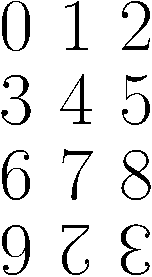
\includegraphics[height=\textheight]{digits-crop.pdf} &%
\fontsize{24pt}{24pt}\selectfont \textit{Let $\sigma_0(n)$ and
		$\sigma_1(n)$ denote the number and sum of the
		divisors of $n$, respectively (i.e., the zeroth- and
		first-order divisor functions).  A number $n$ is
		called sublime if $\sigma_0(n)$ and $\sigma_1(n)$ are
		both perfect numbers.  The only two known sublime
		numbers are [decimal] 12 and [a decimal number with
		decimal 76 digits]  It is not known if any odd sublime
		number exists.}\par\vskip.5em \fontsize{18pt}{18pt}\selectfont \hbox{\textsc{\vbox{\hangafter=0\hangindent=2em%
	Weisstein, Eric W.  "Sublime Number."
		From \textit{MathWorld---A Wolfram Web Resource}.
		\url{http://mathworld.wolfram.com/SublimeNumber.html}.}}}\\%
\end{tabular}%
\end{landscape}%
		\begin{landscape}
		\renewcommand*{\arraystretch}{1.2}
		\vspace{-1em}\centering\monthsty{January 11\e\x}\vskip1em
		\noindent
		\begin{tabular}{|%
			>{\daysty\vspace{-.5em}}p{\daywidth}<{\vspace{-.8em}}|%
			>{\daysty\vspace{-.5em}}p{\daywidth}<{\vspace{-.8em}}|%
			>{\daysty\vspace{-.5em}}p{\daywidth}<{\vspace{-.8em}}|%
			>{\daysty\vspace{-.5em}}p{\daywidth}<{\vspace{-.8em}}|%
			>{\daysty\vspace{-.5em}}p{\daywidth}<{\vspace{-.8em}}|%
			>{\daysty\vspace{-.5em}}p{\daywidth}<{\vspace{-.8em}}|%
			>{\daysty\vspace{-.5em}}p{\daywidth}<{\vspace{-.8em}}|}
		\hline
		Sunday & Monday & Tuesday & Wednesday & Thursday%
		& Friday & Saturday \\
		\end{tabular}\vskip-1.4pt

\renewcommand*{\arraystretch}{1.2}
\noindent
\begin{tabular}{|p{\daywidth}|p{\daywidth}|%
p{\daywidth}|p{\daywidth}|p{\daywidth}|p{\daywidth}|%
p{\daywidth}|}
\hline
\multicolumn{3}{|c|}{
\hbox to 3\daywidth{%

	\hfil\hbox to\daywidth{%

		\vbox to.2\dayheight{\vskip2pt%

			\hbox to\daywidth{\hfil\thumbtitsty%

				December\hfil}\vskip2pt%

			\hbox to\daywidth{\hfil%

				\usebox{\monthunqua}\hfil}%

		}%

	}%

	\hfil\hbox to\daywidth{%

		\vbox to.2\dayheight{\vskip2pt%

			\hbox to\daywidth{\hfil\thumbtitsty%

				February\hfil}\vskip2pt%

			\hbox to\daywidth{\hfil%

				\usebox{\monthunqtwo}\hfil}%

		}%

	}\hfil%

}%

} &
\vtop to\dayheight {\hbox to \linewidth{\hfil\numsty 1\ls}
\rule{0pt}{\dayheight}}&\vtop to\dayheight {\hbox to \linewidth{\hfil\numsty 2\ls}
\rule{0pt}{\dayheight}}&\vtop to\dayheight {\hbox to \linewidth{\hfil\numsty 3\ls}
\rule{0pt}{\dayheight}}&\vtop to\dayheight {\hbox to \linewidth{\hfil\numsty 4\ls}
\rule{0pt}{\dayheight}}\\\hline
\vtop to\dayheight {\hbox to \linewidth{\hfil\numsty 5\ls}
\rule{0pt}{\dayheight}}&\vtop to\dayheight {\hbox to \linewidth{\hfil\numsty 6\ls}
\rule{0pt}{\dayheight}}&\vtop to\dayheight {\hbox to \linewidth{\hfil\numsty 7\ls}
\rule{0pt}{\dayheight}}&\vtop to\dayheight {\hbox to \linewidth{\hfil\numsty 8\ls}
\rule{0pt}{\dayheight}}&\vtop to\dayheight {\hbox to \linewidth{\hfil\numsty 9\ls}
\rule{0pt}{\dayheight}}&\vtop to\dayheight {\hbox to \linewidth{\hfil\numsty \x\ls}
\rule{0pt}{\dayheight}}&\vtop to\dayheight {\hbox to \linewidth{\hfil\numsty \e\ls}
\rule{0pt}{\dayheight}}\\\hline
\vtop to\dayheight {\hbox to \linewidth{\hfil\numsty 10\ls}
\rule{0pt}{\dayheight}}&\vtop to\dayheight {\hbox to \linewidth{\hfil\numsty 11\ls}
\rule{0pt}{\dayheight}}&\vtop to\dayheight {\hbox to \linewidth{\hfil\numsty 12\ls}
\rule{0pt}{\dayheight}}&\vtop to\dayheight {\hbox to \linewidth{\hfil\numsty 13\ls}
\rule{0pt}{\dayheight}}&\vtop to\dayheight {\hbox to \linewidth{\hfil\numsty 14\ls}
\rule{0pt}{\dayheight}}&\vtop to\dayheight {\hbox to \linewidth{\hfil\numsty 15\ls}
\rule{0pt}{\dayheight}}&\vtop to\dayheight {\hbox to \linewidth{\hfil\numsty 16\ls}
\rule{0pt}{\dayheight}}\\\hline
\vtop to\dayheight {\hbox to \linewidth{\hfil\numsty 17\ls}
\rule{0pt}{\dayheight}}&\vtop to\dayheight {\hbox to \linewidth{\hfil\numsty 18\ls}
\rule{0pt}{\dayheight}}&\vtop to\dayheight {\hbox to \linewidth{\hfil\numsty 19\ls}
\rule{0pt}{\dayheight}}&\vtop to\dayheight {\hbox to \linewidth{\hfil\numsty 1\x\ls}
\rule{0pt}{\dayheight}}&\vtop to\dayheight {\hbox to \linewidth{\hfil\numsty 1\e\ls}
\rule{0pt}{\dayheight}}&\vtop to\dayheight {\hbox to \linewidth{\hfil\numsty 20\ls}
\rule{0pt}{\dayheight}}&\vtop to\dayheight {\hbox to \linewidth{\hfil\numsty 21\ls}
\rule{0pt}{\dayheight}}\\\hline
\vtop to\dayheight {\hbox to \linewidth{\hfil\numsty 22\ls}
\rule{0pt}{\dayheight}}&\vtop to\dayheight {\hbox to \linewidth{\hfil\numsty 23\ls}
\rule{0pt}{\dayheight}}&\vtop to\dayheight {\hbox to \linewidth{\hfil\numsty 24\ls}
\rule{0pt}{\dayheight}}&\vtop to\dayheight {\hbox to \linewidth{\hfil\numsty 25\ls}
\rule{0pt}{\dayheight}}&\vtop to\dayheight {\hbox to \linewidth{\hfil\numsty 26\ls}
\rule{0pt}{\dayheight}}&\vtop to\dayheight {\hbox to \linewidth{\hfil\numsty 27\ls}
\rule{0pt}{\dayheight}}&\multicolumn{1}{c|}{
\hbox to 1\daywidth{%

	\hfil\hbox to\daywidth{%

		\vbox to.2\dayheight{\vskip2pt%

			\hbox to\daywidth{\hfil\thumbtitsty%

				February\hfil}\vskip2pt%

			\hbox to\daywidth{\hfil%

				\usebox{\monthunqtwo}\hfil}%

		}%

	}\hfil%

}%

} &
\hline\end{tabular}
\end{landscape}
\newpage
\begin{landscape}%
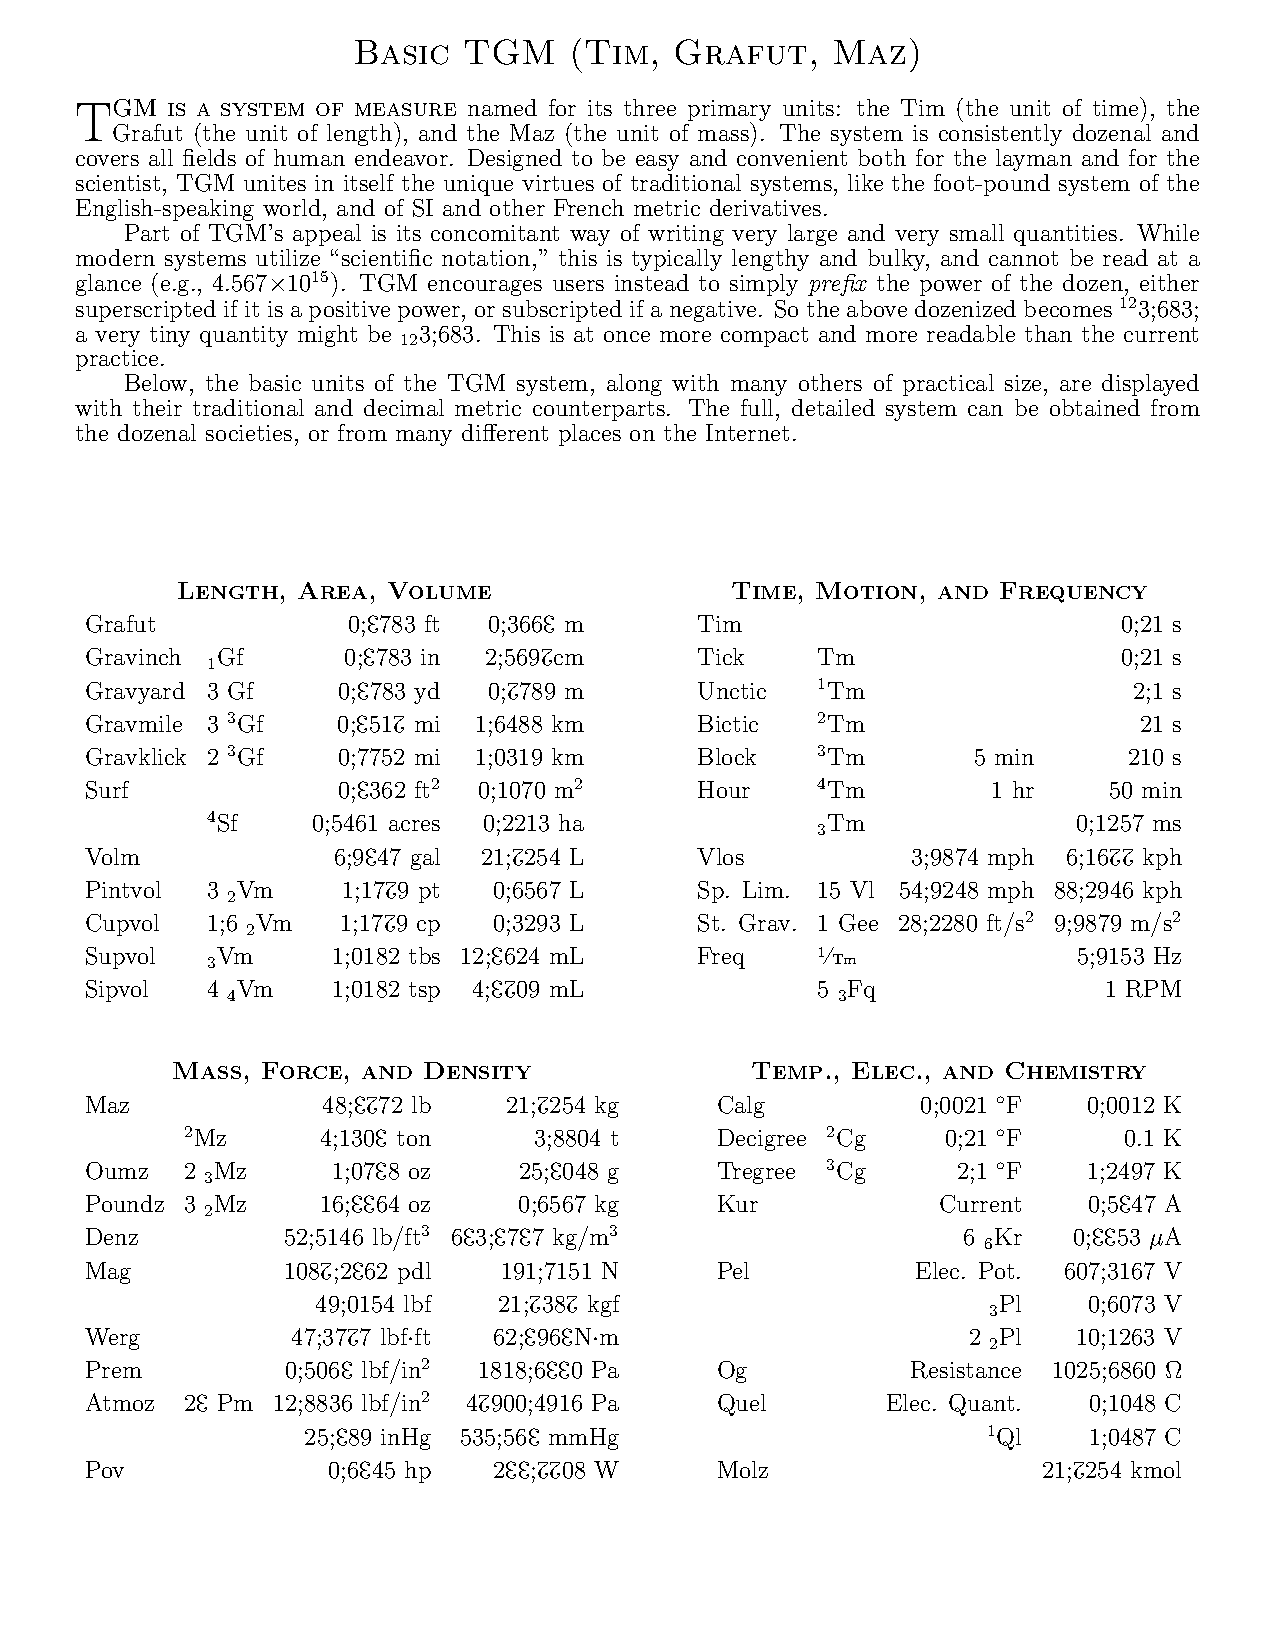
\includepdf[offset=4em 0em,delta=0em -4em,noautoscale,scale=0.70,landscape,turn=false,pages=-,nup=1x2]{closing.pdf}%
\end{landscape}%
\end{document}
